% Options for packages loaded elsewhere
\PassOptionsToPackage{unicode}{hyperref}
\PassOptionsToPackage{hyphens}{url}
\documentclass[
]{article}
\usepackage{xcolor}
\usepackage[margin=0.78in]{geometry}
\usepackage{amsmath,amssymb}
\setcounter{secnumdepth}{-\maxdimen} % remove section numbering
\usepackage{iftex}
\ifPDFTeX
  \usepackage[T1]{fontenc}
  \usepackage[utf8]{inputenc}
  \usepackage{textcomp} % provide euro and other symbols
\else % if luatex or xetex
  \usepackage{unicode-math} % this also loads fontspec
  \defaultfontfeatures{Scale=MatchLowercase}
  \defaultfontfeatures[\rmfamily]{Ligatures=TeX,Scale=1}
\fi
\usepackage{lmodern}
\ifPDFTeX\else
  % xetex/luatex font selection
\fi
% Use upquote if available, for straight quotes in verbatim environments
\IfFileExists{upquote.sty}{\usepackage{upquote}}{}
\IfFileExists{microtype.sty}{% use microtype if available
  \usepackage[]{microtype}
  \UseMicrotypeSet[protrusion]{basicmath} % disable protrusion for tt fonts
}{}
\makeatletter
\@ifundefined{KOMAClassName}{% if non-KOMA class
  \IfFileExists{parskip.sty}{%
    \usepackage{parskip}
  }{% else
    \setlength{\parindent}{0pt}
    \setlength{\parskip}{6pt plus 2pt minus 1pt}}
}{% if KOMA class
  \KOMAoptions{parskip=half}}
\makeatother
\usepackage{longtable,booktabs,array}
\newcounter{none} % for unnumbered tables
\usepackage{calc} % for calculating minipage widths
% Correct order of tables after \paragraph or \subparagraph
\usepackage{etoolbox}
\makeatletter
\patchcmd\longtable{\par}{\if@noskipsec\mbox{}\fi\par}{}{}
\makeatother
% Allow footnotes in longtable head/foot
\IfFileExists{footnotehyper.sty}{\usepackage{footnotehyper}}{\usepackage{footnote}}
\makesavenoteenv{longtable}
\usepackage{graphicx}
\makeatletter
\newsavebox\pandoc@box
\newcommand*\pandocbounded[1]{% scales image to fit in text height/width
  \sbox\pandoc@box{#1}%
  \Gscale@div\@tempa{\textheight}{\dimexpr\ht\pandoc@box+\dp\pandoc@box\relax}%
  \Gscale@div\@tempb{\linewidth}{\wd\pandoc@box}%
  \ifdim\@tempb\p@<\@tempa\p@\let\@tempa\@tempb\fi% select the smaller of both
  \ifdim\@tempa\p@<\p@\scalebox{\@tempa}{\usebox\pandoc@box}%
  \else\usebox{\pandoc@box}%
  \fi%
}
% Set default figure placement to htbp
\def\fps@figure{htbp}
\makeatother
\setlength{\emergencystretch}{3em} % prevent overfull lines
\providecommand{\tightlist}{%
  \setlength{\itemsep}{0pt}\setlength{\parskip}{0pt}}
\usepackage{bookmark}
\IfFileExists{xurl.sty}{\usepackage{xurl}}{} % add URL line breaks if available
\urlstyle{same}
% fallback for those not using the hyperref driver hyperxmp:
\makeatletter
\@ifundefined{xmpquote}{\newcommand{\xmpquote}[1]{#1}}{}
\makeatother
\hypersetup{
  pdftitle={Runtime Pass Is Not Correctness},
  pdfauthor={George Pu},
  hidelinks,
  pdfcreator={LaTeX via pandoc}}

\ifXeTeX
\special{pdf:trailerid [ <69659651b77959bb620ddb464f487242> <69659651b77959bb620ddb464f487242> ]}
\fi
\ifPDFTeX
\pdftrailerid{}
\pdftrailer{/ID [ <69659651b77959bb620ddb464f487242> <69659651b77959bb620ddb464f487242> ]}
\fi
\ifLuaTeX
\pdfvariable trailerid {[ <69659651b77959bb620ddb464f487242> <69659651b77959bb620ddb464f487242> ]}
\fi

\title{Runtime Pass Is Not Correctness}
\usepackage{etoolbox}
\makeatletter
\providecommand{\subtitle}[1]{% add subtitle to \maketitle
  \apptocmd{\@title}{\par {\large #1 \par}}{}{}
}
\makeatother
\subtitle{A Negative Reasoning-Efficiency Post-Training Result and
Verifier Audit on Qwen3.8-27B}
\author{George Pu}
\date{1 September 2026}

\begin{document}
\maketitle

{
\setcounter{tocdepth}{3}
\tableofcontents
}
\begin{quote}
\textbf{Unpublished corrected candidate --- package revision 1.0.3.}
This repository-forward derivative has not been published, tagged,
uploaded to Zenodo, or submitted to arXiv. The published v1.0 PDF
remains a frozen historical artifact and contains residual
pre-finalization instructions that are corrected in this candidate.
\end{quote}

\subsection{Abstract}\label{abstract}

Reasoning-capable language models can consume large inference budgets
without delivering a usable answer. P-BREVE-01-R2 tested whether a small
supervised fine-tuning (SFT) stage followed by conservative
length-debiased Direct Preference Optimization (DPO) could make
\texttt{Qwen/Qwen3.8-27B} allocate reasoning effort more proportionally,
terminate reliably, preserve correct delivery, and avoid learning a
global ``shorter is better'' rule. The intervention used a BF16 rank-32
LoRA, 440 accepted SFT demonstrations, 700 accepted DPO pairs, and a
frozen two-seed development evaluation. The original evaluation bank
contained 400 tasks across direct, closed-form, executable-code,
agentic, and answerability strata.

The configured one-epoch SFT-to-DPO recipe did not meet its
pre-registered efficiency objectives. Throughout this report,
\textbf{reasoning reduction versus base is signed so that positive
values mean fewer tokens and negative values mean more tokens}. On that
metric, the one-epoch SFT+DPO arm scored \textbf{−10.9\% at seed 1729
(longer than base)} and \textbf{+4.9\% at seed 2718 (shorter than
base)}, against a required \textbf{+20\% reduction at both seeds}. The
marginal reasoning reduction from adding DPO after SFT was −0.6\% and
+0.6\%, providing no evidence of a meaningful one-epoch DPO effect. That
one-epoch result was negative on oracle-independent efficiency measures
before the later evaluator audit; it was not an apparent gain that was
subsequently withdrawn. A bounded two-epoch screen produced an apparent
dose response on executable-code token and cap-exhaustion measures under
the study's \texttt{reasoning\_effort=xhigh} serving condition. A
subsequent serving-control experiment showed that changing untrained
base weights from \texttt{xhigh} to the neutral \texttt{medium} setting
moved executable-code cap exhaustion from 65\% to 0\% on the screened
shard and reduced restricted mean reasoning length from 6,407 to 608
tokens. The formal matched-effort comparison remained underpowered, but
the result was sufficient to show that the \textbf{two-epoch dose
response} could not be attributed cleanly to trained weights. The
adapter was retired and no checkpoint was selected for release.

The stronger finding came from auditing the evaluator. The original
executable-code bank accepted 24 of 24 deliberately incorrect shortcut
programs, including branches that returned the expected output from
input length without reading input values. Its 80 nominal code tasks
represented eight content-distinct problems cloned ten times, and its
apparent capability residual included specification-ambiguous tasks.
Correctness claims dependent on that bank were therefore withdrawn or
suspended; raw token and termination measurements were retained only
within their narrower scope.

A replacement 40-task runtime/certification design improved
discrimination but remained unqualified. The visible runtime channel
accepted 154 of 322 broad shortcut probes, while the protected
certification channel accepted none of those 322. Certification
nevertheless accepted 7 of 157 near-miss or partial programs, and the
frozen grader rejected 7 of the bank's 40 correct reference
implementations because of a non-behavioural abstract-syntax
restriction. A later independently constructed mutation population
generated 1,862 provably wrong mutants; 52 passed certification, with at
least one leak in 19 of 40 protected tasks. The cross-method
affected-task lower bound was composed explicitly as \textbf{seven
previously identified Defect-B tasks plus fourteen newly adjudicated
tasks outside that set, yielding at least 21 of 40 tasks with a known
certification flaw}. This union count is distinct from the same source
document's complementary statement that 21 of 40 tasks showed no leak
under the mutation population alone.

P-BREVE-01-R2 is therefore a negative model-intervention result and a
positive evaluator-audit result. It supports three bounded conclusions:
the configured conservative SFT+DPO recipe did not establish a
training-attributable reasoning-efficiency improvement; serving-time
effort controls dominated the observed termination phenotype on the
screened code tasks; and executable success is not evidence of
correctness until the evaluator has survived independent shortcut,
near-miss, valid-alternative, independence, censoring, and power checks.
The report distills those failures into \textbf{Vinci Eval Integrity
0.1}, a seven-check admission record covering statistical identity,
contract clarity, channel separation, bidirectional discrimination,
estimand integrity, production-path binding, and power with independent
post-repair requalification. No model, bank, or release candidate
resulted from the study.

\textbf{Keywords:} reasoning efficiency; overthinking; Direct Preference
Optimization; executable evaluation; verifier validity; reward hacking;
mutation testing; hidden tests; negative results; open-weight language
models

\textbf{Publication record.} Version 1.0; research evidence cutoff
\texttt{7cdfb4b68b7265be7f6c7299b107ff9d924f2a2d} (private research
repository \texttt{getsimpledirect/vinci-gpu-research}, program
directory \texttt{p-breve-01-r2/}); canonical report page:
\href{https://www.getsimpledirect.com/research/papers/runtime-pass-is-not-correctness}{\url{https://www.getsimpledirect.com/research/papers/runtime-pass-is-not-correctness}}.
The evidence cutoff is a research-record identity, not a claim that
every execution manifest contained a Git commit.

\pandocbounded{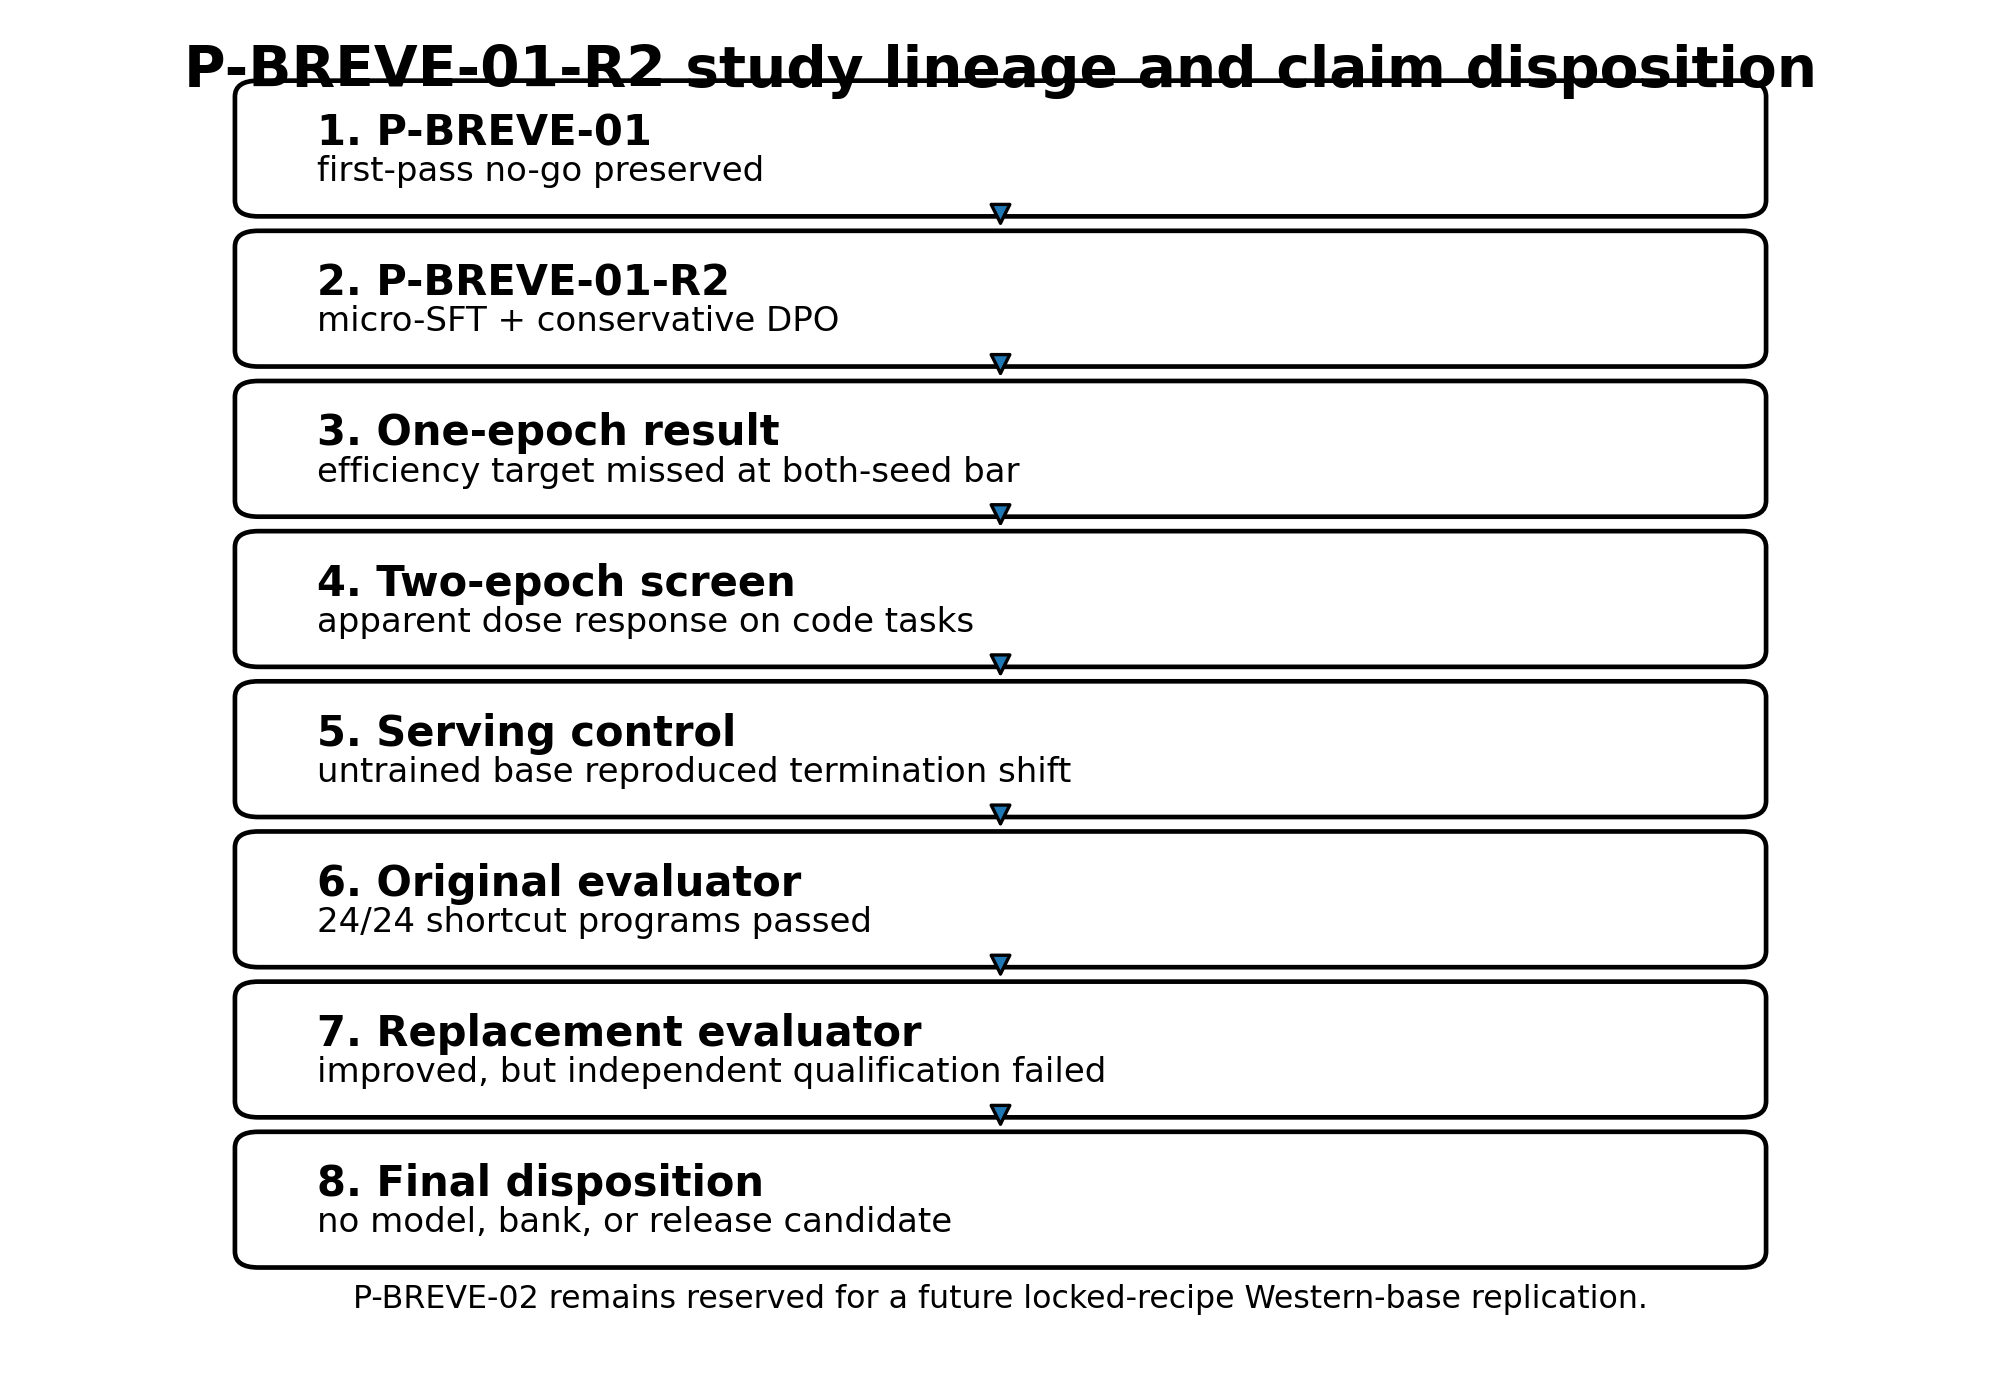
\includegraphics[keepaspectratio,alt={Figure 1. Study lineage and final disposition. P-BREVE-01 remains a preserved no-go; P-BREVE-01-R2 produced a negative intervention result, a serving-control confound, and evaluator-audit findings. No model, bank, or release candidate resulted.}]{figures/figure1_study_lineage.png}}

\subsection{1. Introduction}\label{1-introduction}

Large reasoning models can improve difficult-task performance by
generating long intermediate traces, but the same mechanism can spend
substantial compute on unnecessary reconsideration, repeat already
completed derivations, or reach a generation limit before returning a
usable final answer. This creates a practical optimization problem:
reduce waste without suppressing the reasoning that difficult tasks
genuinely require.

Recent work attacks this problem through adaptive inference policies,
learned stopping signals, optimal-stopping controllers, and per-step
effort routers {[}3--6{]}. These approaches share an important
requirement. A system may only stop earlier when the shorter trajectory
still delivers the correct outcome. Token reduction alone is not an
adequate objective. A model that stops by refusing, guessing,
truncating, skipping verification, or exploiting an incomplete evaluator
can appear efficient while becoming less useful.

P-BREVE-01-R2 studied a weight-level intervention rather than a
stand-alone inference controller. The intended policy was
task-conditional:

\begin{itemize}
\tightlist
\item
  easy tasks should receive brief or empty reasoning and an exact
  requested final;
\item
  closed-form problems should receive one sufficient derivation rather
  than repeated derivation;
\item
  executable-code tasks should receive a verified implementation in the
  requested output format;
\item
  agentic tasks should use tools, consume feedback, and verify the
  resulting state before declaring completion;
\item
  unanswerable tasks should identify missing information rather than
  guess, loop, or exhaust the token budget; and
\item
  genuinely hard tasks should retain sufficient depth.
\end{itemize}

The intervention combined small SFT with conservative DPO. SFT
established the desired response grammar and examples of proportional
reasoning. DPO then preferred less redundant trajectories only where
both candidates independently satisfied the same task authority;
guardrail pairs preferred correct and verified responses over shorter
but defective alternatives. More than half of accepted pairs
deliberately had a chosen response that was not shorter than the
rejected response. The design was intended to make correctness outrank
length.

The primary research question was:

\begin{quote}
Can micro-SFT followed by conservative length-debiased DPO improve
Qwen3.8-27B's reasoning allocation, final-channel discipline, and
verified delivery without replacing reasoning with generic brevity,
refusal, or unverified action?
\end{quote}

The study initially appeared to produce a mixed answer. The one-epoch
recipe failed its efficiency target, while a stronger dose appeared to
reduce code-stratum reasoning and cap exhaustion. Further controls then
showed that the serving harness itself injected an \texttt{xhigh}
reasoning instruction, and that changing the untrained base model to a
neutral effort setting reproduced or exceeded the termination
improvement. The trained effect was no longer identifiable from the
apparent dose response.

More consequentially, the correctness evaluator failed adversarial
qualification. A verifier can be deterministic, content-addressed,
reproducible, and wrong. The original bank ran code and returned stable
results, but its tests did not distinguish general implementations from
trivial programs specialized to the small visible input set. It also
counted repeated variants of eight underlying problems as 80 independent
tasks. These defects did not merely add uncertainty to the reported
accuracy. They changed what the number meant.

This report therefore makes five contributions.

First, it reports a bounded negative result for the configured one-epoch
SFT+DPO intervention. Second, it separates an apparent two-epoch dose
response from a serving-control effect and explains why the adapter was
retired. Third, it demonstrates a concrete failure of executable
verification: 24 of 24 adversarial non-solutions passed the original
code bank. Fourth, it reports the strengths and remaining failures of a
replacement runtime/certification design across broad shortcuts,
near-miss programs, valid alternatives, and an independently constructed
mutation population. Fifth, it documents the claim-withdrawal and
correction process---including which measurements remain interpretable
and which do not---and distills the resulting requirements into
\textbf{Vinci Eval Integrity 0.1}, a seven-check evaluator-admission
record.

The result is not a model launch. It does not establish that preference
optimization cannot improve reasoning efficiency, that Qwen3.8-27B
generally overthinks, that safety was preserved, or that the replacement
bank is qualified. It establishes that this recipe did not earn its
intended claim and that the measurement system required deeper
qualification than the original program had imposed.

\subsection{2. Related Work}\label{2-related-work}

\subsubsection{2.1 Adaptive reasoning and early
stopping}\label{21-adaptive-reasoning-and-early-stopping}

Difficulty-adaptive inference provides a direct alternative to
weight-level post-training. DiffAdapt selects among easy, normal, and
hard inference strategies using a lightweight difficulty probe and
reports token reductions of up to 22.4\% while maintaining comparable or
improved benchmark performance {[}3{]}. ESTAR learns self-generated
stopping signals and combines SFT with stop-aware reinforcement
learning; its reported experiments reduce average reasoning length from
4,799 to 1,290 tokens while preserving similar accuracy {[}4{]}.
OS-Pruner formulates chain-of-thought truncation as an optimal-stopping
problem and reports generation-length reductions of 20--60\% with
limited accuracy loss {[}5{]}. Ares chooses reasoning effort per step in
multi-step agents and reports reductions of up to 52.7\% in reasoning
tokens with limited task-success degradation {[}6{]}.

These systems differ in training requirements and control granularity,
but all make the same conceptual move: reasoning effort should depend on
evidence about the task rather than remain globally fixed. P-BREVE-01-R2
began from the same principle. Its failure to isolate a weight-level
effect, together with the strength of the \texttt{medium} serving
control, pushes the evidence toward controller-first investigation
rather than stronger preference tuning on the same base.

\subsubsection{2.2 Direct Preference Optimization and length
control}\label{22-direct-preference-optimization-and-length-control}

DPO provides a supervised classification objective for fitting a policy
to pairwise preferences relative to a reference model, avoiding a
separately trained reward model and an online reinforcement-learning
loop {[}2{]}. In reasoning-efficiency work, however, the preference
relation is easy to misspecify. If shorter responses are usually labeled
preferred, a policy can learn generic brevity rather than
task-conditional efficiency. Conversely, if guardrail examples dominate
without any within-task efficiency contrast, the dataset may protect
correctness while supplying too little gradient toward reduced waste.

P-BREVE-01-R2 used two explicit pair types. Efficiency pairs required
both branches to pass the same authority before preferring the less
redundant one. Guardrail pairs preferred correct, complete, and verified
responses over guesses, truncations, format violations, answerable
refusals, or unverified agent actions. The accepted set contained 218
efficiency pairs and 482 guardrail pairs; 56.6\% of chosen branches were
not shorter than their rejected alternatives. This prevented a simple
corpus-level ``always shorter'' rule, but the corpus still contained no
efficiency pairs for the executable-code or agentic-decision-state
families. That defect is relevant to interpretation, although it does
not explain the complete result: the strata with explicit efficiency
pairs did not show the intended gain, while the code stratum without
such pairs produced the largest apparent dose response under
\texttt{xhigh}.

\subsubsection{2.3 Executable rewards, public tests, and reward
hacking}\label{23-executable-rewards-public-tests-and-reward-hacking}

Code-generation systems often treat passing tests as an objective
measure of correctness. That interpretation depends on the tests.
Insufficient coverage can create false-positive rewards and encourage
policies to exploit visible cases rather than satisfy the underlying
specification. RobustTests explicitly uses faulty programs to synthesize
cases that expose logical gaps in code rewards {[}7{]}. SWE-Mutation
evaluates generated test suites by measuring whether systematically
mutated programs can still pass, and reports low detection rates for
current models on realistic agent-generated mutants {[}8{]}. CodeAssay
combines audited references, public and hidden tests, and mutation-based
validation; auditing changed 9.0\% of fixed-output correctness labels in
its reported experiment {[}9{]}.

Reward-hacking benchmarks show that the issue is not hypothetical.
BAITBENCH places optional shortcuts in machine-learning tasks that
inflate a public metric while failing hidden evaluation and reports
reward-hacking behaviour in 57.1\% of tested frontier-agent runs
{[}10{]}. The relevance to P-BREVE is structural rather than identical:
a program can maximize the observable proxy while violating the intended
task, and the proxy itself may not reveal the violation.

\subsubsection{2.4 Mutation testing as evaluator
qualification}\label{24-mutation-testing-as-evaluator-qualification}

Mutation testing evaluates a test suite by introducing controlled faults
and measuring which faults the suite detects {[}11{]}. Applied to model
evaluation, it asks a more useful question than whether the reference
solution passes: does the evaluator reject programs that are wrong in
plausible, specification-relevant ways, while continuing to accept
legitimate alternatives?

P-BREVE's initial audit used human-designed shortcut and near-miss
programs. A later audit generated first-order abstract-syntax-tree
mutations from the reference implementations and admitted only mutants
that demonstrably disagreed with the reference on generated inputs.
Neither method was exhaustive. Their value came from finding different
defects. The combined record shows why evaluator qualification cannot
rely on one mutation family, one author, or one repair population.

\subsection{3. Study Lineage and
Protocol}\label{3-study-lineage-and-protocol}

\subsubsection{3.1 P-BREVE-01 and the R2 recovery
study}\label{31-p-breve-01-and-the-r2-recovery-study}

P-BREVE-01 was an earlier bounded study on the same pinned Qwen3.8-27B
substrate. Its revised first-pass gate ended in a no-go before training.
That result remains closed and unchanged. P-BREVE-01-R2 was created as a
narrower recovery study focused on task-conditional stopping, exact
final-channel discipline, and verified agentic behaviour.

The identifier matters. R2 is not \texttt{P-BREVE-02}. The original
charter reserves \texttt{P-BREVE-02} for a future locked-recipe
reproduction on a Western 24--32B base. The present report covers the
Qwen recovery lineage only and does not consume that future identifier.

\subsubsection{3.2 Evidence tier and report
cutoff}\label{32-evidence-tier-and-report-cutoff}

All model results in this report are development-tier internal evidence.
No sealed primary product-weighted holdout was opened, no external peer
review was performed, and no independent external laboratory reproduced
the result. Several evaluator audits were designed and run after defects
were discovered rather than before the model experiment. They are
valuable diagnostic evidence, not confirmatory evidence about a
pre-registered auditor hypothesis.

\subsubsection{3.3 Model and serving
stack}\label{33-model-and-serving-stack}

The frozen substrate was \texttt{Qwen/Qwen3.8-27B} at revision {[}1{]}:

\texttt{1d4bf0f2ff6012fd82039f2fa52739d0dd7c60c0}

Training used BF16 weights and adapters without quantization. Evaluation
ran on the Vinci H200 fleet using the pinned Qwen chat template and a
vLLM-based serving path. The final adapter was served attached rather
than merged. In an eight-fixture parity test, BF16 merging produced
token-identical greedy output on only five fixtures and consequential
divergence on one cap-truncated fixture. Adapter-attached serving was
therefore designated the canonical evidence path.

The pinned chat template exposed a serving variable that became central
to the result. \texttt{reasoning\_effort=xhigh} injected a
natural-language instruction to think carefully, validate assumptions,
and consider alternatives. \texttt{medium} injected no effort-specific
instruction and served as the neutral baseline. \texttt{low} injected a
brief-reasoning instruction. An absent effort value resolved to
\texttt{xhigh}.

\subsubsection{3.4 Intervention}\label{34-intervention}

The intervention was frozen as follows.

{\def\LTcaptype{none} % do not increment counter
\begin{longtable}[]{@{}p{0.48\linewidth}p{0.23\linewidth}p{0.23\linewidth}@{}}
\toprule\noalign{}
Component & SFT & DPO \\
\midrule\noalign{}
\endhead
\bottomrule\noalign{}
\endlastfoot
Accepted examples & 440 demonstrations & 700 preference pairs \\
Precision & BF16 & BF16 \\
Adapter & LoRA rank 32, alpha 64, dropout 0.05 & continued from accepted
SFT adapter \\
Epochs & 1 & 1 in the primary configured recipe \\
Learning rate & \texttt{1e-5} & \texttt{5e-6} \\
Schedule & cosine, 3\% warmup & frozen training configuration \\
Maximum complete sequence length & 8,192 & 8,192 per branch \\
Quantization & none & none \\
DPO beta & --- & 0.10 \\
Length coefficient & --- & 0.05 \\
Reference policy & --- & exact accepted SFT checkpoint \\
\end{longtable}
}

SFT loss applied only to assistant reasoning, final-answer, and
tool-call tokens. System, user, and tool-result tokens were masked. DPO
prompts and tool-result spans were likewise masked. Silent truncation
was prohibited.

\subsubsection{3.5 Data construction and
acceptance}\label{35-data-construction-and-acceptance}

The data program generated 2,000 rollout rows from a declared 600-prompt
training-only pool plus inherited, re-verified anchors. The accepted SFT
and DPO artifacts were assembled only after schema, hash, authority,
overlap, and family-balance checks. Unknown outcomes were quarantined
rather than interpreted as passes.

The accepted DPO set contained two classes:

{\def\LTcaptype{none} % do not increment counter
\begin{longtable}[]{@{}p{0.48\linewidth}p{0.18\linewidth}p{0.28\linewidth}@{}}
\toprule\noalign{}
Pair type & Count & Intended function \\
\midrule\noalign{}
\endhead
\bottomrule\noalign{}
\endlastfoot
Efficiency & 218 & Both branches pass the same authority; prefer less
redundant reasoning or a cleaner final contract \\
Guardrail & 482 & Prefer correct, complete, verified behaviour over
shorter but defective behaviour \\
\textbf{Total} & \textbf{700} & \\
\end{longtable}
}

The chosen response was not shorter in 56.6\% of accepted pairs.
Guardrail pairs represented 68.9\% of the corpus. These properties made
a corpus-wide length shortcut less attractive, but they did not
guarantee that each semantic family carried a useful efficiency
gradient.

\subsubsection{3.6 Original evaluation
bank}\label{36-original-evaluation-bank}

The frozen R2-G4 development bank contained 400 nominal tasks:

{\def\LTcaptype{none} % do not increment counter
\begin{longtable}[]{@{}p{0.72\linewidth}p{0.22\linewidth}@{}}
\toprule\noalign{}
Stratum & Nominal tasks \\
\midrule\noalign{}
\endhead
\bottomrule\noalign{}
\endlastfoot
Direct/easy & 80 \\
Closed-form & 80 \\
Executable code & 80 \\
Agentic tool use & 80 \\
Answerability & 80 \\
\textbf{Total} & \textbf{400} \\
\end{longtable}
}

Base and adapter conditions were evaluated on matched tasks under two
fixed inference seeds, 1729 and 2718. Each arm therefore contained 800
episodes. The base-versus-adapter comparison contained 1,600 matched
episodes.

The original positive-efficiency gates required, at both seeds:

\begin{itemize}
\tightlist
\item
  at least 20\% lower median reasoning tokens;
\item
  at least 15\% lower median total generated tokens;
\item
  at least 15\% lower agentic generated tokens including retries;
\item
  no increase in cap exhaustion or severe degeneration; and
\item
  no material regression in correctness, final validity, answerable
  refusal, tool serialization, or safety outcomes.
\end{itemize}

Correctness-dependent gates are reported here only as historical design
requirements. After the executable-code bank failed adversarial
qualification, they could no longer support model-level conclusions.

\subsubsection{3.7 Bounded dose and serving-control
screens}\label{37-bounded-dose-and-serving-control-screens}

After the one-epoch recipe failed, the program authorized one bounded
dose-response test from the same SFT checkpoint and the same 700 pairs.
The DPO dose changed from one to two epochs. The evaluation data and
serving condition remained fixed.

A later six-arm serving-control screen crossed checkpoint identity with
effort configuration:

{\def\LTcaptype{none} % do not increment counter
\begin{longtable}[]{@{}p{0.34\linewidth}p{0.28\linewidth}p{0.32\linewidth}@{}}
\toprule\noalign{}
Arm & Checkpoint & Effort \\
\midrule\noalign{}
\endhead
\bottomrule\noalign{}
\endlastfoot
A1 & Base & \texttt{xhigh} \\
A2 & Base & \texttt{medium} \\
A3 & Base & \texttt{low} \\
A4 & Base & thinking disabled \\
A5 & Two-epoch DPO & \texttt{xhigh} \\
A6 & Two-epoch DPO & \texttt{medium} \\
\end{longtable}
}

The screen used one shared 100-episode shard: 50 nominal tasks, two
decoding seeds, and 20 episodes per stratum. It was explicitly
underpowered for a five-point strict-success non-inferiority claim. Its
formal decision state was \texttt{INDETERMINATE}.

\subsubsection{3.8 Artifact and claim
governance}\label{38-artifact-and-claim-governance}

Training, serving, and evaluation artifacts were content-addressed and
bound to model, template, adapter, bank, schedule, and authority
identities. The program maintained an append-only claims registry with
states including exploratory, development-supported, contradicted, and
suspended. This became important after an evaluator audit changed which
portions of earlier claims remained interpretable.

The completed full-recipe G4 result, measured on 18--19 August 2026, is
now represented by claim \path{pbr2.g4.full-recipe-insufficient.015}.
The claim was registered late on 1 September without new measurement. It
preserves the oracle-independent token and termination findings while
excluding the raw-code strict rate from interpretation because the bank
was condemned. The same record cleanup distinguishes two different arm
sets: the sealed Stage-3 base/intervention pair was never dispatched,
whereas the R2-G4 full-recipe evaluation completed. The registry does
not currently encode a distinct ``partially narrowed'' state. This
report therefore defines a publication-local disposition,
\textbf{retained, narrowed}, for a result whose evidentiary core
survives only after a named unsupported component is removed. The label
does not mutate or override the registry.

Content addressing prevented silent rewriting, but it did not guarantee
semantic correctness. Several later findings involved the right digest
over the wrong authority, the right source file with stale bytecode
executing, or a fully reproducible test suite that accepted incorrect
programs. Reproducibility and validity were therefore treated as
separate properties.

\pandocbounded{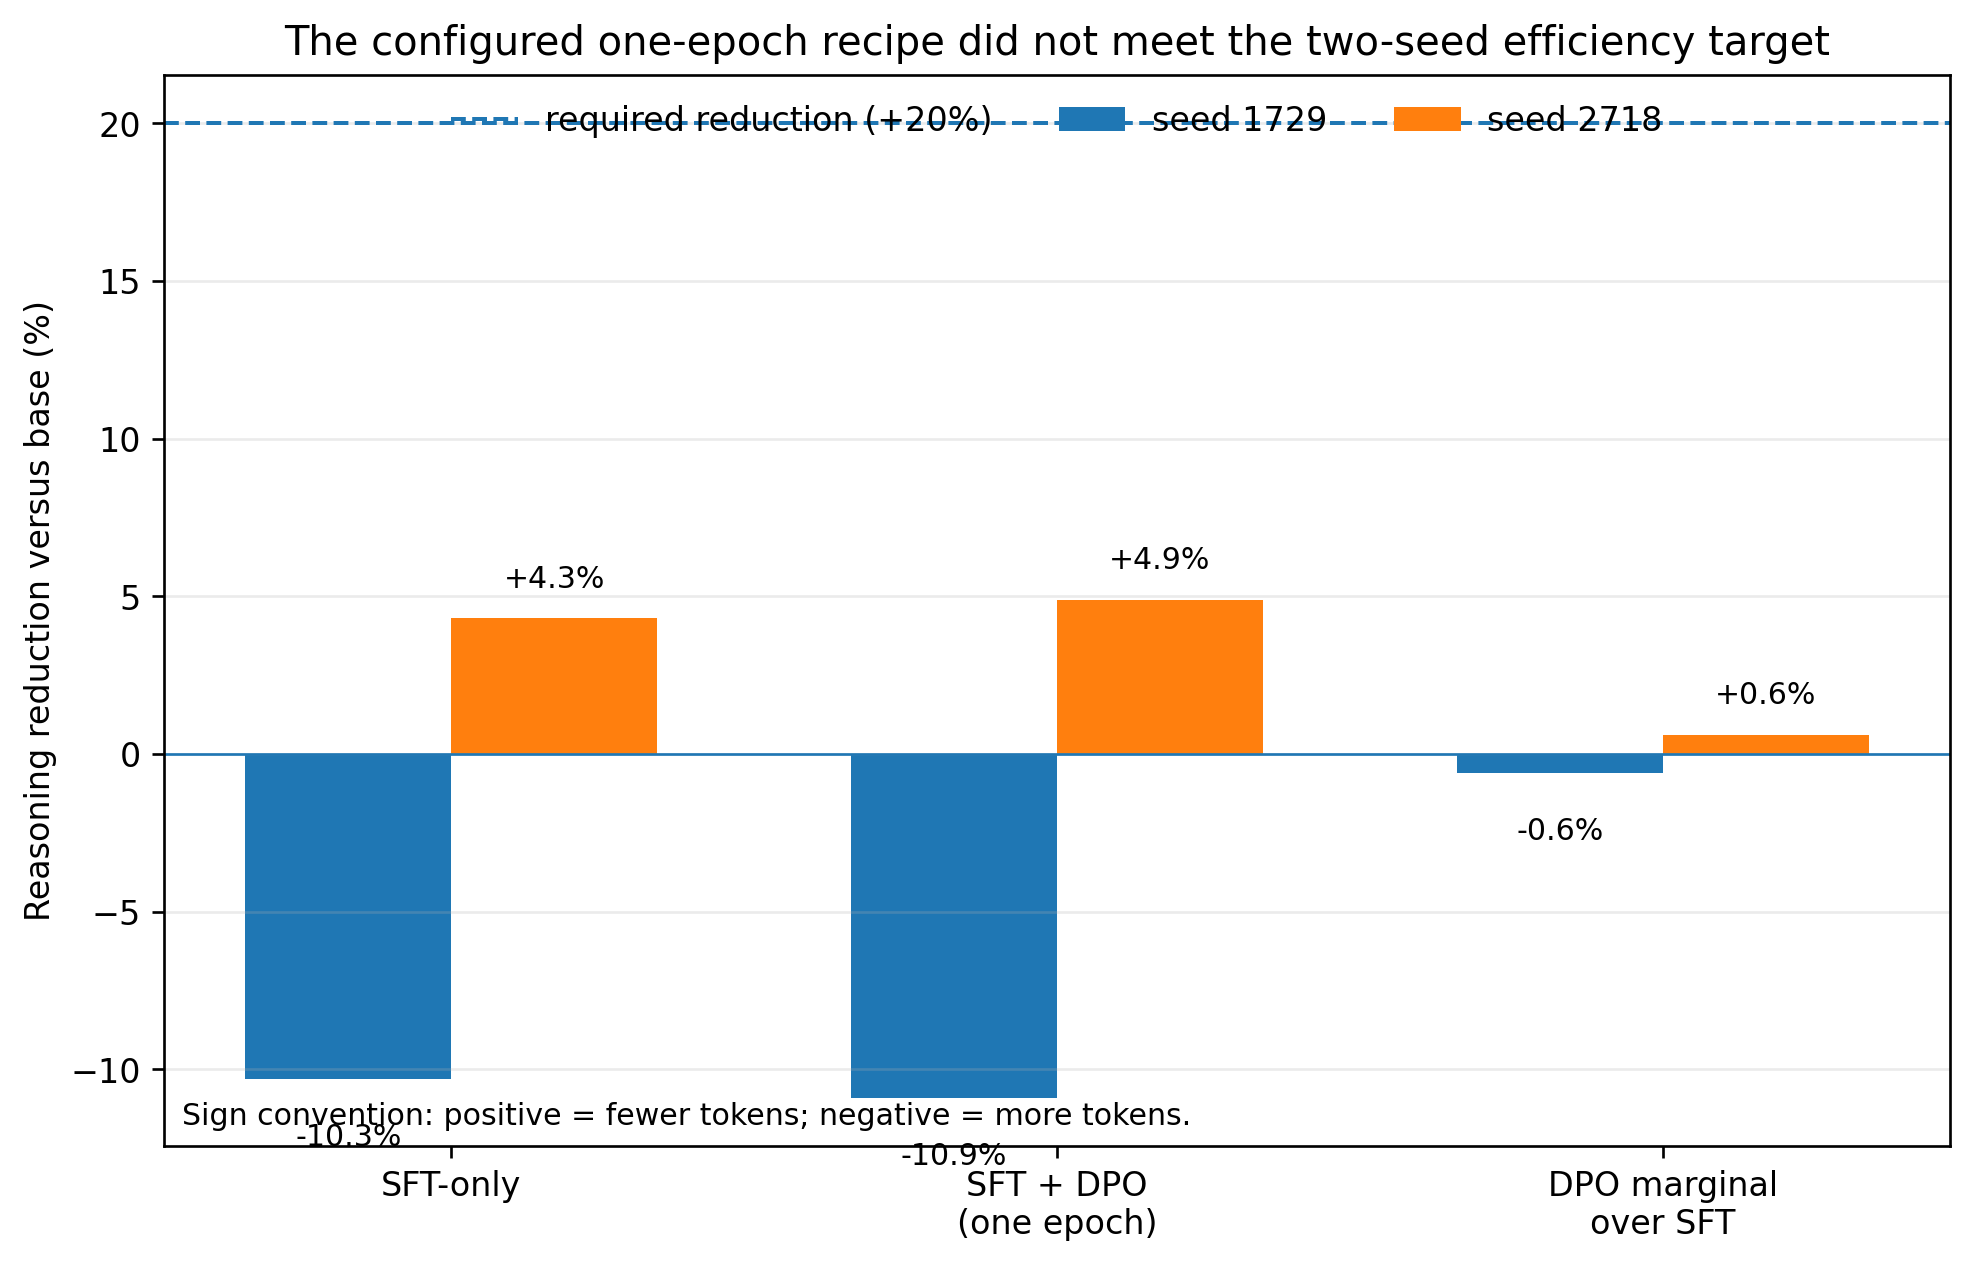
\includegraphics[keepaspectratio,alt={Figure 2. Signed one-epoch reasoning reduction. Positive values mean fewer tokens and negative values mean more tokens. The full recipe missed the required +20\% reduction at both seeds.}]{figures/figure2_one_epoch_reduction.png}}

\subsection{4. Results}\label{4-results}

\subsubsection{4.1 The intervention executed, but execution was not the
scientific
endpoint}\label{41-the-intervention-executed-but-execution-was-not-the-scientific-endpoint}

The accepted training package contained 440 SFT demonstrations and 700
DPO pairs. All eight rollout shards completed and the accepted sets
passed the program's internal schema, authority, balance, and
content-addressing gates. The training path also encountered several
first-contact failures that are relevant because they show the
difference between a pipeline that eventually executes and a result that
was valid from the beginning.

The first SFT smoke found that the pinned Qwen chat template carried no
generation markers compatible with the initial masking implementation.
The implementation therefore produced an all-zero assistant-loss mask on
every row. A fail-closed mask audit rejected the run before a GPU
training step occurred. The repaired, byte-anchored template
augmentation was then checked across all 440 accepted rows, yielding
119,146 assistant loss tokens with no prompt or tool-result loss and a
maximum sequence length of 8,167 within the 8,192-token limit.

The DPO path subsequently completed 44 optimization steps. The recorded
loss moved from approximately 0.693 at initialization to 0.376 at the
final checkpoint. That fact establishes that the configured objective
executed and changed the adapter. It does not establish that the
intended behavioural policy was learned.

Serving identity also required a decision. Merging the adapter into BF16
base weights changed greedy generation on three of eight parity
fixtures. Two divergences converged to the same final answer, while one
remained consequentially divergent at the fixture's generation limit.
The attached-adapter path was therefore frozen as the canonical
evaluation artifact. The merged checkpoint had no evidentiary role.

These controls matter, but they should not be confused with the result.
The report's scientific question is not whether a LoRA was trained,
whether loss declined, or whether the evaluation jobs returned exit code
zero. It is whether the intervention produced a task-conditional
efficiency improvement under a valid measurement instrument.

\subsubsection{4.2 The configured one-epoch SFT-to-DPO recipe missed
every positive-efficiency
target}\label{42-the-configured-one-epoch-sft-to-dpo-recipe-missed-every-positive-efficiency-target}

The primary configured recipe compared the frozen base, the accepted SFT
adapter, and the one-epoch SFT+DPO adapter on the same nominal 400-task
bank under two fixed inference seeds. The original decision packet
contained correctness, safety, and formatting outcomes alongside token
measurements. After the code verifier was condemned, only
oracle-independent quantities remained interpretable. Table 1 therefore
reports reasoning, generation, and termination quantities only.

\textbf{Table 1. Oracle-independent outcomes for the configured
one-epoch recipe. A positive reduction means fewer tokens than base.
Displayed token medians are rounded; percentage changes reproduce the
frozen scorer from underlying records and therefore need not equal
ratios of the displayed integers exactly.}

{\def\LTcaptype{none} % do not increment counter
\begin{longtable}[]{@{}p{0.34\linewidth}p{0.20\linewidth}p{0.20\linewidth}p{0.20\linewidth}@{}}
\toprule\noalign{}
Metric & Seed 1729 & Seed 2718 & Frozen target \\
\midrule\noalign{}
\endhead
\bottomrule\noalign{}
\endlastfoot
Base median reasoning tokens & 156 & 184 & --- \\
SFT median reasoning tokens & 172 & 176 & --- \\
SFT+DPO median reasoning tokens & 172 & 175 & --- \\
SFT+DPO reasoning reduction vs. base & \textbf{−10.9\% (longer)} &
\textbf{+4.9\% (shorter)} & \textbf{at least +20\% at both seeds} \\
DPO marginal reasoning reduction vs. SFT & \textbf{−0.6\%} &
\textbf{+0.6\%} & positive trained contribution \\
SFT+DPO total-generated-token reduction vs. base & +8.6\% & -1.8\% & at
least +15\% at both seeds \\
Base cap-exhaustion rate & 12.8\% & 13.2\% & --- \\
SFT+DPO cap-exhaustion rate & 10.2\% & 12.0\% & no increase; reduction
desirable \\
\end{longtable}
}

The recipe failed the reasoning-reduction target at both seeds. At seed
1729 it increased the median reasoning length. At seed 2718 it reduced
the median by less than one quarter of the required amount. Total
generated tokens also failed the two-seed target. Most importantly for
identifying the contribution of preference optimization, the one-epoch
DPO stage moved median reasoning by approximately zero relative to SFT
alone.

The cap-exhaustion point estimate fell by 2.6 percentage points at seed
1729 and 1.2 points at seed 2718. Those are valid termination
measurements, but they do not rescue the intervention. The positive
contract was not ``slightly fewer cap hits somewhere in the bank.'' It
required a material, two-seed reduction in reasoning and total
generation while preserving verified delivery.

The bounded conclusion is therefore negative:

\begin{quote}
Under the frozen data, one-epoch SFT, one-epoch conservative
length-debiased DPO, \texttt{xhigh} serving condition, and development
task distribution, the intervention did not produce a material or
reproducible reasoning-efficiency improvement, and the marginal
contribution of DPO over SFT was approximately zero.
\end{quote}

This conclusion does not imply that DPO cannot affect reasoning length,
that another data distribution would fail, or that another model lineage
would behave identically. It rejects the configured recipe at the
evidence tier and thresholds actually used.

\subsubsection{\texorpdfstring{4.3 A stronger DPO dose produced an
apparent code-stratum response under
\texttt{xhigh}}{4.3 A stronger DPO dose produced an apparent code-stratum response under xhigh}}\label{43-a-stronger-dpo-dose-produced-an-apparent-code-stratum-response-under-xhigh}

After the one-epoch null, the program authorized one bounded dose test.
The SFT checkpoint, 700 DPO pairs, objective, adapter scope, and
evaluation bank were held fixed; DPO epochs increased from one to two.

At the pooled-bank level, the two-epoch arm's signed reasoning reduction
versus base was \textbf{+10.9\% at seed 1729} and \textbf{+24.5\% at
seed 2718}. It therefore still failed the frozen requirement of at least
+20\% at both seeds. The sign and arm label are deliberate: at seed
1729, the one-epoch arm was \textbf{−10.9\%} while the two-epoch arm was
\textbf{+10.9\%}---equal magnitudes in opposite directions. The more
informative exploratory pattern appeared in the executable-code stratum,
where more than half of episodes were censored at the 8,192-token
reasoning limit.

\textbf{Table 2. Executable-code token and termination measurements
under \texttt{reasoning\_effort=xhigh}.}

{\def\LTcaptype{none} % do not increment counter
\begin{longtable}[]{@{}p{0.48\linewidth}p{0.23\linewidth}p{0.23\linewidth}@{}}
\toprule\noalign{}
Arm & p25 reasoning tokens & Observed cap-exhaustion rate \\
\midrule\noalign{}
\endhead
\bottomrule\noalign{}
\endlastfoot
Base & 5,359 & 63.7\% \\
SFT+DPO, 1 epoch & 3,628 & 55.6\% \\
SFT+DPO, 2 epochs & 2,604 & 48.8\% \\
\end{longtable}
}

The p25 and cap-exhaustion measures moved monotonically with DPO dose.
Four other strata had p25 reasoning values around 48--60 tokens and
moved little. Under the frozen serving condition, the effect therefore
looked task-conditional rather than like indiscriminate shortening.

That finding was initially summarized as evidence that ``dose is the
lever.'' It was later withdrawn as a trained-model interpretation for
two reasons. First, the correctness instrument was invalid, so the
accompanying claims about recovered coding capability were unsupported.
Second, the experiment had held a consequential serving instruction
fixed at \texttt{xhigh}. The dose series showed how different
checkpoints behaved while all were being instructed to reason at the
highest effort. It did not establish that trained weights were the
source of the termination improvement.

The raw measurements in Table 2 remain part of the record. The causal
interpretation does not.

\subsubsection{4.4 A serving control reproduced the termination
improvement on untrained
weights}\label{44-a-serving-control-reproduced-the-termination-improvement-on-untrained-weights}

The pinned Qwen chat template did not treat \texttt{reasoning\_effort}
as passive metadata. At \texttt{xhigh}, it injected a natural-language
instruction telling the model to reason carefully, validate assumptions,
and consider alternatives. At \texttt{medium}, it injected no
effort-specific instruction. At \texttt{low}, it instructed the model to
reason briefly. If no value was provided, the template resolved to
\texttt{xhigh}.

The six-arm control screen evaluated the base and two-epoch DPO
checkpoints on one shared 100-episode shard. The executable-code stratum
contained 20 episodes representing ten nominal tasks under two decoding
seeds. Because those repeated seeds were clustered within tasks, the
screen was underpowered for the pre-registered five-point correctness
margin. Its formal verdict remained \texttt{INDETERMINATE}.

Termination and reasoning-cost differences were nevertheless large.

\textbf{Table 3. Executable-code serving-control screen. RMST is
restricted mean reasoning length at the frozen cap. Zero observed cap
hits means 0 of 20 episodes, not a population rate of exactly zero.}

{\def\LTcaptype{none} % do not increment counter
\begin{longtable}[]{@{}p{0.34\linewidth}p{0.20\linewidth}p{0.20\linewidth}p{0.20\linewidth}@{}}
\toprule\noalign{}
Checkpoint and effort & Observed cap hits & Cap-exhaustion rate & RMST,
reasoning tokens \\
\midrule\noalign{}
\endhead
\bottomrule\noalign{}
\endlastfoot
Base @ \texttt{xhigh} & 13/20 & 0.65 & 6,407 \\
Base @ \texttt{medium} & 0/20 & 0.00 & 608 \\
Base @ \texttt{low} & 0/20 & 0.00 & 449 \\
Base @ thinking disabled & 0/20 & 0.00 & 0 \\
Two-epoch DPO @ \texttt{xhigh} & 8/20 & 0.40 & 5,103 \\
Two-epoch DPO @ \texttt{medium} & 0/20 & 0.00 & 579 \\
\end{longtable}
}

Changing untrained base weights from \texttt{xhigh} to \texttt{medium}
reduced observed cap exhaustion by 65 percentage points and RMST by
5,799 tokens. At matched \texttt{medium}, the base and DPO arms had
nearly identical termination profiles: 0 of 20 observed cap hits and
RMST values of 608 and 579 tokens. The matched-effort design could not
establish strict-success non-inferiority at its sample size, and
correctness point estimates from the condemned bank are not used here.
The screen therefore does not prove that the adapter had exactly zero
behavioural effect.

It does establish a more limited but decision-relevant fact: the
apparent trained benefit under \texttt{xhigh} was not identifiable as a
weight effect because a serving-only change reproduced nearly the entire
observed termination improvement on untrained weights. Continuing to
increase DPO dose before treating the serving policy as the comparator
would have optimized around an avoidable harness choice.

This control did \textbf{not} change the one-epoch verdict, which was
already negative on the token and termination endpoints. It changed the
attribution of the \textbf{two-epoch} response: the raw measurements
remain, while the interpretation that dose had established a
trained-weight benefit was withdrawn.

The two-epoch adapter was retired. No checkpoint from the lineage was
designated a model or product candidate.

\pandocbounded{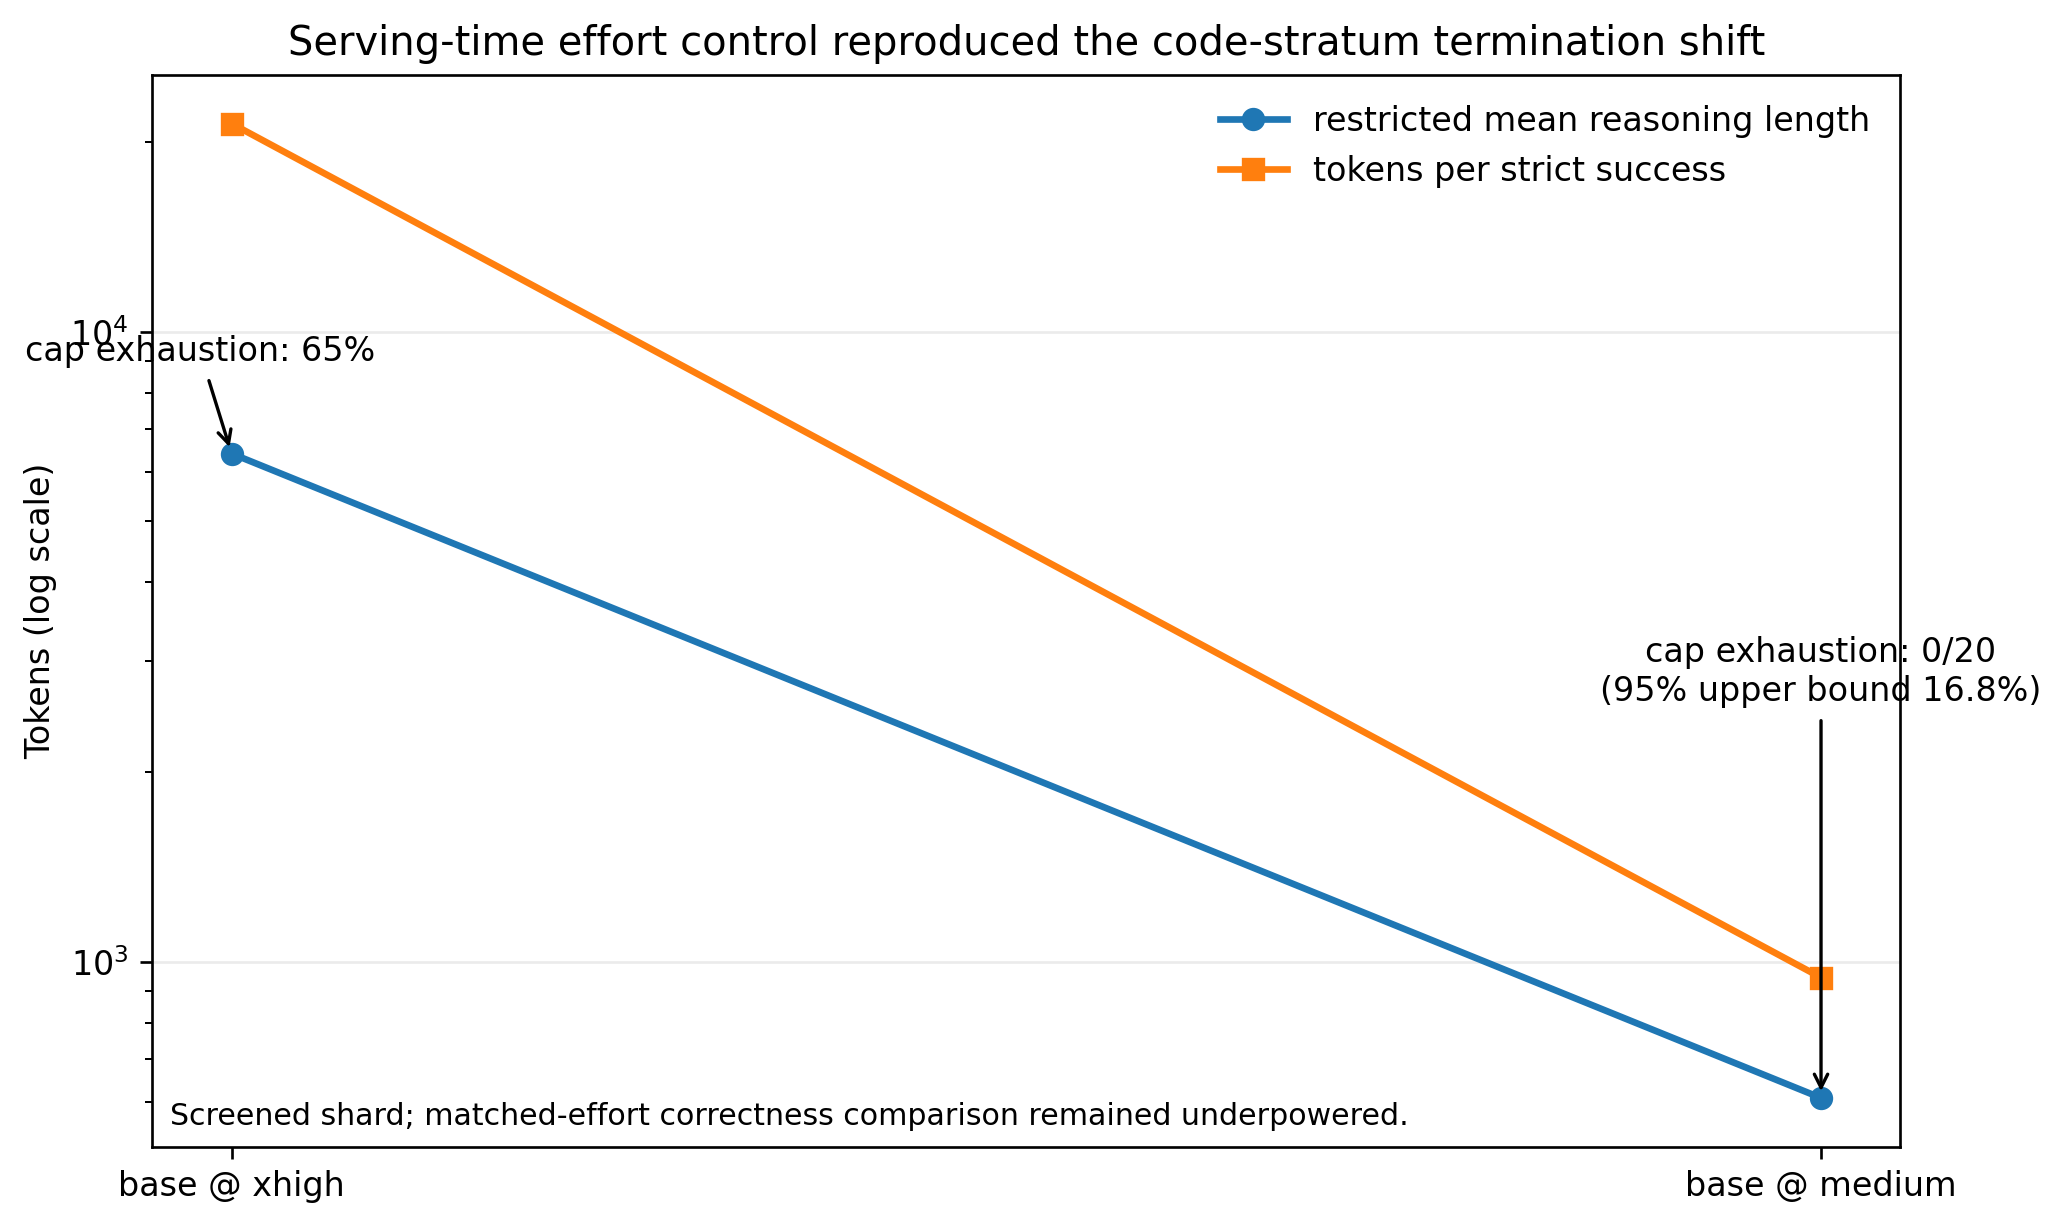
\includegraphics[keepaspectratio,alt={Figure 3. Serving-time effort control. On the screened executable-code shard, changing untrained base weights from xhigh to medium moved cap exhaustion from 65\% to 0/20 and sharply reduced token consumption. The matched-effort correctness comparison remained underpowered.}]{figures/figure3_serving_effort_control.png}}

\subsubsection{4.5 The original executable-code evaluator accepted every
broad shortcut
attack}\label{45-the-original-executable-code-evaluator-accepted-every-broad-shortcut-attack}

The evaluator audit covered 26 tasks spanning all eight content-distinct
executable-code families. It graded 562 candidate programs through the
frozen authority, including adversarial shortcuts, plausible
alternatives, near-miss mutants, metamorphic rewrites, and repeated
executions.

The headline result was decisive:

\begin{quote}
\textbf{All 24 broad adversarial non-solutions passed: 24/24, exact 95\%
confidence interval {[}0.858, 1.000{]}.}
\end{quote}

Three attacks were constructed for each semantic family.

\textbf{Table 4. Broad shortcut probes against the original bank.}

{\def\LTcaptype{none} % do not increment counter
\begin{longtable}[]{@{}p{0.48\linewidth}p{0.30\linewidth}p{0.16\linewidth}@{}}
\toprule\noalign{}
Probe class & Behaviour & Result \\
\midrule\noalign{}
\endhead
\bottomrule\noalign{}
\endlastfoot
Literal lookup & Maps the three known inputs directly to expected
outputs & 8/8 families passed \\
Incidental-scalar branch & Selects an answer from one argument value
that happens to identify the case & 8/8 passed \\
Shape or fingerprint branch & Selects an answer from \texttt{len},
\texttt{sum}, or another aggregate without implementing the task & 8/8
passed \\
\textbf{Total} & & \textbf{24/24 passed} \\
\end{longtable}
}

The most revealing probe branched only on input length. Each family's
three cases had different lengths, so length uniquely identified the
expected output. The program did not need to inspect a single element of
the input. The evaluator executed ordinary Python, observed the expected
values, and returned success.

The bank had a second structural defect. Its 80 nominal executable-code
tasks were eight content-distinct problems cloned ten times. Function
names and task identifiers differed, but prompts normalized for the
entrypoint and test bodies were identical within each family. Treating
the 80 task identifiers as independent observations overstated the
information in the sample. Under the limiting case of perfect
within-family correlation, standard errors could be understated by
approximately the square root of ten, or 3.16 times. The exact
correction depends on the statistic and within-family correlation; 3.16
is a limiting comparison, not an estimated intraclass-correlation
adjustment.

The apparent residual capability failures were also not stable task
properties. Two residual families admitted defensible interpretations
that the hidden tests rejected. In one, the prompt described parameters
\texttt{a} and \texttt{b} on a ring of size \texttt{n}, while the tests
called the function in the order \texttt{(n,\ a,\ b)}. A correct
implementation following the prompt's own naming order scored 0 of 3.
Matched clones of the same prompt and tests appeared on both sides of
the ``solved'' and ``unresolved'' split, showing that the split could
not be attributed to task or verifier content.

The instrument was not indiscriminate in every direction. Thirty-five
independently written valid alternative implementations were accepted,
repeated clean-sandbox executions showed 0 of 40 family-level flakes,
and metamorphic rewrites showed 0 of 40 disagreements. Near-miss testing
still found four false acceptances in 32 family-level probes. These
results are useful because they show the actual failure mode. The
evaluator was stable and permissive toward legitimate implementation
diversity, but its case sets did not distinguish the task from broad
shortcuts and some explicit requirement violations.

A deterministic wrong instrument remains wrong. The following
consequences were adopted:

\begin{itemize}
\tightlist
\item
  absolute executable-code correctness rates from the original bank were
  withdrawn;
\item
  relative correctness rankings were not assumed safe, because verifier
  error might differ by policy;
\item
  the fixed-policy correctness frontier was suspended;
\item
  the bank was prohibited as an executable reward for optimization or
  reinforcement learning; and
\item
  the nominal 80-task unit was replaced by semantic-family-aware
  accounting.
\end{itemize}

Single-shot model generations had not been optimized against these
tests, so the audit does not establish that the evaluated model
intentionally exploited the reward. It establishes that the score could
not distinguish genuine correctness from a readily reachable
non-solution.

\subsubsection{4.6 A runtime/certification split improved broad-shortcut
rejection but remained
unqualified}\label{46-a-runtimecertification-split-improved-broad-shortcut-rejection-but-remained-unqualified}

The replacement design separated two functions that the original bank
had collapsed:

\begin{itemize}
\tightlist
\item
  \textbf{Runtime tests} were small, visible, and intended only to
  decide whether a system should accept, retry, or repair an attempt.
\item
  \textbf{Certification tests} were protected, larger, supplemented with
  seeded generated cases, and intended to determine the scientific
  score.
\end{itemize}

The 40-task batch-2 bank was audited with 577 probes, of which 563 were
scored and 14 were excluded because no behavioural difference from the
reference could be established.

\textbf{Count-rendering convention.} Slash-form counts are treated as
derived quantities even when the source report prints the same ratio.
Here \texttt{154/322} means the runtime channel's
\texttt{shortcuts\ that\ pass} count divided by the broad-shortcut
population for families 1--5. The \texttt{7/157} certification count
combines the near-miss and partial families and can be re-derived as
\texttt{(4\ +\ 3)\ /\ (121\ +\ 36)}. Version 1.0 verified these fields
in \texttt{p-breve-01-r2/docs/VERIFIER-QUALIFICATION-BATCH2.md} at
working commit \texttt{7cdfb4b68b7265be7f6c7299b107ff9d924f2a2d}, file
blob \texttt{0d8164fe70d6e770b65f0eb18c6707c2c6255ba1}. Appendix A
records the formulas so publication binding covers both source cells and
rendered ratios.

\textbf{Table 5. Qualification results for the batch-2
runtime/certification design.}

{\def\LTcaptype{none} % do not increment counter
\begin{longtable}[]{@{}p{0.48\linewidth}p{0.23\linewidth}p{0.23\linewidth}@{}}
\toprule\noalign{}
Population or quantity & Runtime channel & Certification channel \\
\midrule\noalign{}
\endhead
\bottomrule\noalign{}
\endlastfoot
Broad shortcuts, families 1--5 & \textbf{154/322 passed (47.8\%)} &
\textbf{0/322 passed (0\%)} \\
Near-miss and partial programs, families 6--7 & reported within audit &
\textbf{7/157 passed (4.5\%)} \\
Established legitimate alternatives, family 8 & --- & \textbf{0/84
falsely rejected} \\
Correct bank reference programs rejected by frozen AST authority &
affected before behavioural execution & \textbf{7/40 rejected
(17.5\%)} \\
`P(certification pass & runtime pass)` on the designed probe population
& --- \\
\end{longtable}
}

The split worked against the attack that destroyed the original bank.
Nearly half of the broad shortcuts passed the visible runtime cases, but
none survived certification. This is the expected role of certification,
not evidence that the runtime layer should be strengthened until it
duplicates the hidden scorer. A small visible test suite is useful for
iteration and inherently exploitable as an optimization target. It must
not be treated as the reward.

The conditional probability of 0.216 also requires careful
interpretation. The probe population was deliberately dominated by wrong
programs. It is not an estimate that 78.4\% of real policy outputs
accepted at runtime would fail in deployment. It demonstrates
non-redundancy: certification added substantial discrimination beyond
runtime on the population designed to test it.

The bank still failed qualification in two directions.

First, seven near-miss or partial programs passed every certification
case. The failures concentrated at boundary conditions, tie-breaking
requirements, empty inputs, and conjunctions of individually covered
edge cases. The certification generator was effective against broad
fingerprinting and weak against rare discriminating instances.

Second, the frozen abstract-syntax authority rejected seven of the
bank's own correct reference programs before execution because they
declared module-level constants. That was a false-rejection mechanism
based on form rather than behaviour. The 0/84 legitimate-alternative
figure did not measure this path because those alternatives had been
authored within the authority's allowed form.

A claim record initially stated the seven-reference result
backwards---as seven tasks accepting non-solutions---because a summary
was copied without opening the audit artifact. The record was later
marked \texttt{contradicted} and superseded by the correctly directed
claim. That correction is included here because it demonstrates the
danger of summarizing a bidirectional verifier audit without naming the
direction of each error.

\subsubsection{4.7 Independent mutation populations showed that targeted
repairs did not
generalize}\label{47-independent-mutation-populations-showed-that-targeted-repairs-did-not-generalize}

\pandocbounded{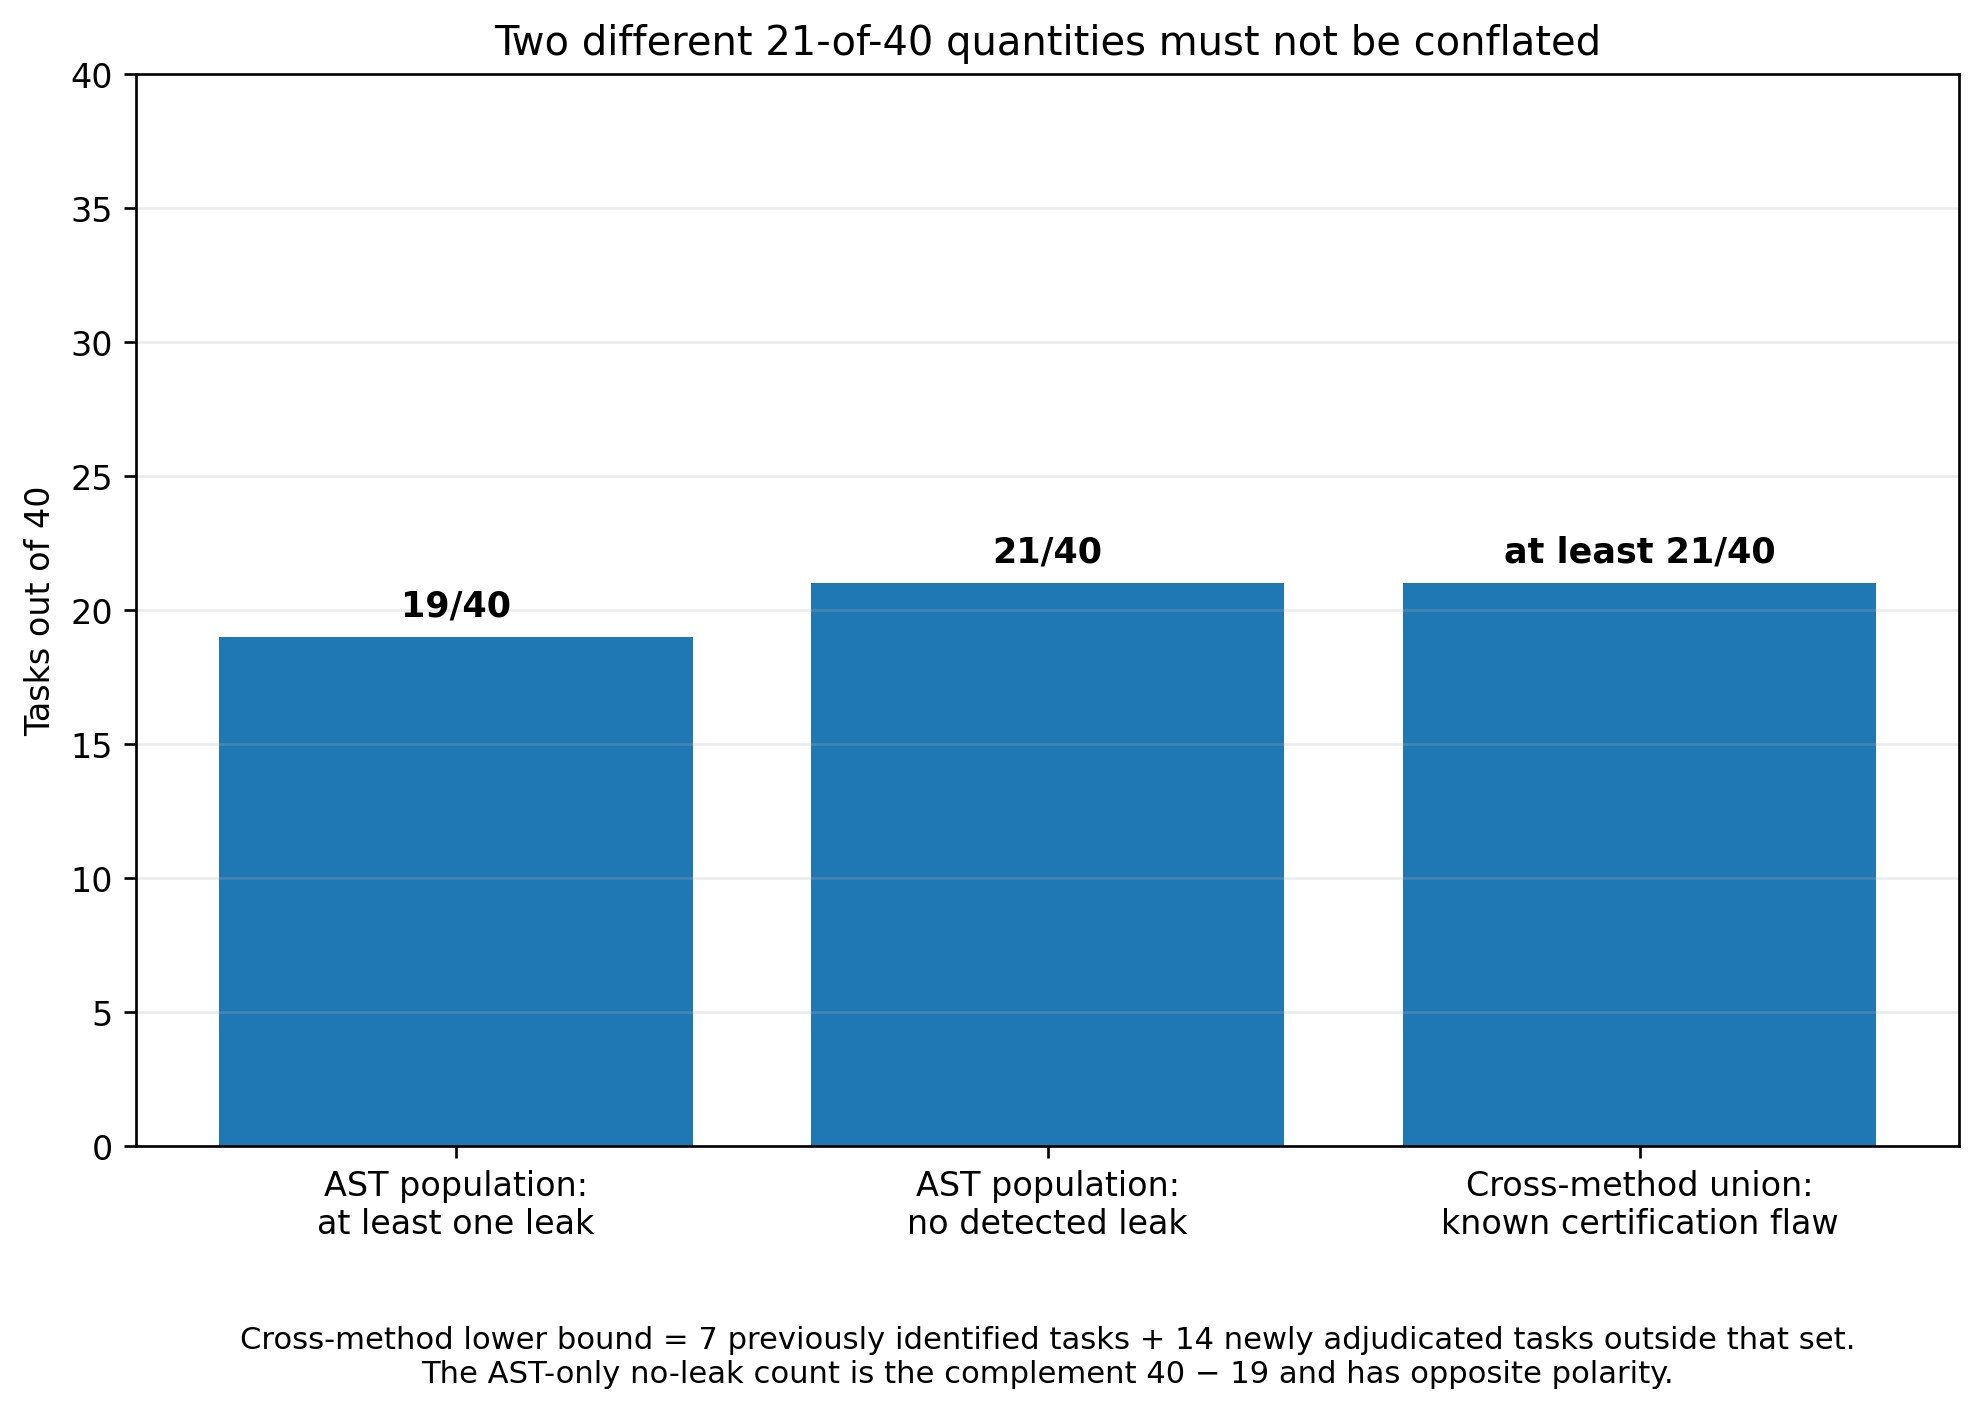
\includegraphics[keepaspectratio,alt={Figure 5. Task-count disambiguation. Nineteen of forty tasks leaked under the AST population, leaving a complementary twenty-one with no detected AST leak; separately, seven prior tasks plus fourteen newly adjudicated tasks establish a cross-method lower bound of at least twenty-one known-flaw tasks.}]{figures/figure5_task_count_disambiguation.png}}

A first repair wave added certification cases derived from the witnessed
near-miss failures. The specific mutants were then caught. A later audit
deliberately changed the way failures were generated: it exhaustively
applied first-order abstract-syntax mutations to reference programs,
admitted only mutants that were provably wrong on generated inputs, and
used controls to show that the tool could produce both zero-leak and
non-zero-leak outcomes.

On the 20-task staging bank after targeted repair, the independent
population generated 1,099 provably wrong mutants. Twenty-three passed
certification across 11 tasks. Adjudication against the prompt contract
classified all 23 as genuine defects, and the 23 programs represented 17
distinct missing certification gaps.

The same unchanged mutation process was then applied to the 40-task
protected batch-2 bank.

\textbf{Table 6. Blind mutation qualification.}

{\def\LTcaptype{none} % do not increment counter
\begin{longtable}[]{@{}p{0.48\linewidth}p{0.23\linewidth}p{0.23\linewidth}@{}}
\toprule\noalign{}
Quantity & Batch-3 staging & Batch-2 protected \\
\midrule\noalign{}
\endhead
\bottomrule\noalign{}
\endlastfoot
Tasks & 20 & 40 \\
Provably wrong mutants & 1,099 & 1,862 \\
Mutants accepted by certification & 23 & 52 \\
Pooled false-accept rate & 2.09\% & 2.79\% \\
Tasks with at least one leak & 11/20 & 19/40 \\
Distinct certification gaps & 17 & 33 \\
\end{longtable}
}

\textbf{Source and derivation record for the protected-bank counts:}
\path{p-breve-01-r2/docs/BLIND-ADVERSARIAL-POPULATION.md}, section
``The protected bank leaks worse than staging.'' Version 1.0 verified
the source at evidence-cutoff commit
\texttt{7cdfb4b68b7265be7f6c7299b107ff9d924f2a2d}, file blob
\texttt{1bb4ea390b38eb4f90d1519933b4e850ede93065}. The report rendering
\texttt{52/1,862} is derived from the adjacent protected-bank cells
\texttt{accepted\ by\ certification\ =\ 52} and
\texttt{provably-wrong\ mutants\ =\ 1,862}; it is not a separately
stored observation. The repository-forward package binds that source
identity in \texttt{data/evidence\_bindings.json} and the rendered
numerator, denominator, rate, and derivation in
\texttt{data/evaluator\_metrics.json}.

The affected-task lower bound is a set union, not a complement and not
the mutation count alone. The witness-driven method had previously
identified seven Defect-B tasks. The AST population implicated 19 tasks,
including fourteen tasks outside that original seven-task set; one
mutation from each of those fourteen was independently adjudicated as a
genuine defect. The cross-method union is therefore:

{[} \textbar W \textbackslash cup M\textbar{} = \textbar W\textbar{} +
\textbar M \textbackslash setminus W\textbar{} = 7 + 14 = 21. {]}

The source document also contains another correct \texttt{21\ of\ 40}
with the opposite polarity: because the AST population found leaks in 19
tasks, \textbf{21 of 40 showed no leak under that population}. The two
counts must never appear without qualifiers.

\textbf{Table 6A. Disambiguating the two \texttt{21/40} counts.}

{\def\LTcaptype{none} % do not increment counter
\begin{longtable}[]{@{}p{0.48\linewidth}p{0.18\linewidth}p{0.28\linewidth}@{}}
\toprule\noalign{}
Label used in this report & Derivation & Meaning \\
\midrule\noalign{}
\endhead
\bottomrule\noalign{}
\endlastfoot
\textbf{AST-leak tasks: 19/40} & directly counted & At least one
provably wrong first-order AST mutant passed certification \\
\textbf{AST-no-leak tasks: 21/40} & \texttt{40\ −\ 19} & No leak was
detected by this mutation population; this is not evidence that the task
is defect-free \\
\textbf{Cross-method known-flaw union: at least 21/40} &
\texttt{7\ previously\ identified\ +\ 14\ newly\ adjudicated\ outside\ that\ set}
& A known certification flaw was established by at least one of the two
non-exhaustive methods \\
\end{longtable}
}

Neither method is exhaustive, so the cross-method 21 is a lower bound on
affected tasks, not an estimate of total defect prevalence.

The result exposes a common repair failure. Adding a case that kills one
mutant proves that mutant is gone. It does not prove the underlying
defect class is closed. A repair population derived from the same
witnesses can certify its own patch. Post-repair qualification needs a
population built by an independent method, and that independent
population must itself carry positive and negative discrimination
controls.

This finding terminated the standalone 15-case repair proposal. The
cases remained correct and necessary, but they were insufficient. No
protected-bank mutation was authorized, and no subsequent model
evaluation could proceed as though batch 2 were qualified.

\pandocbounded{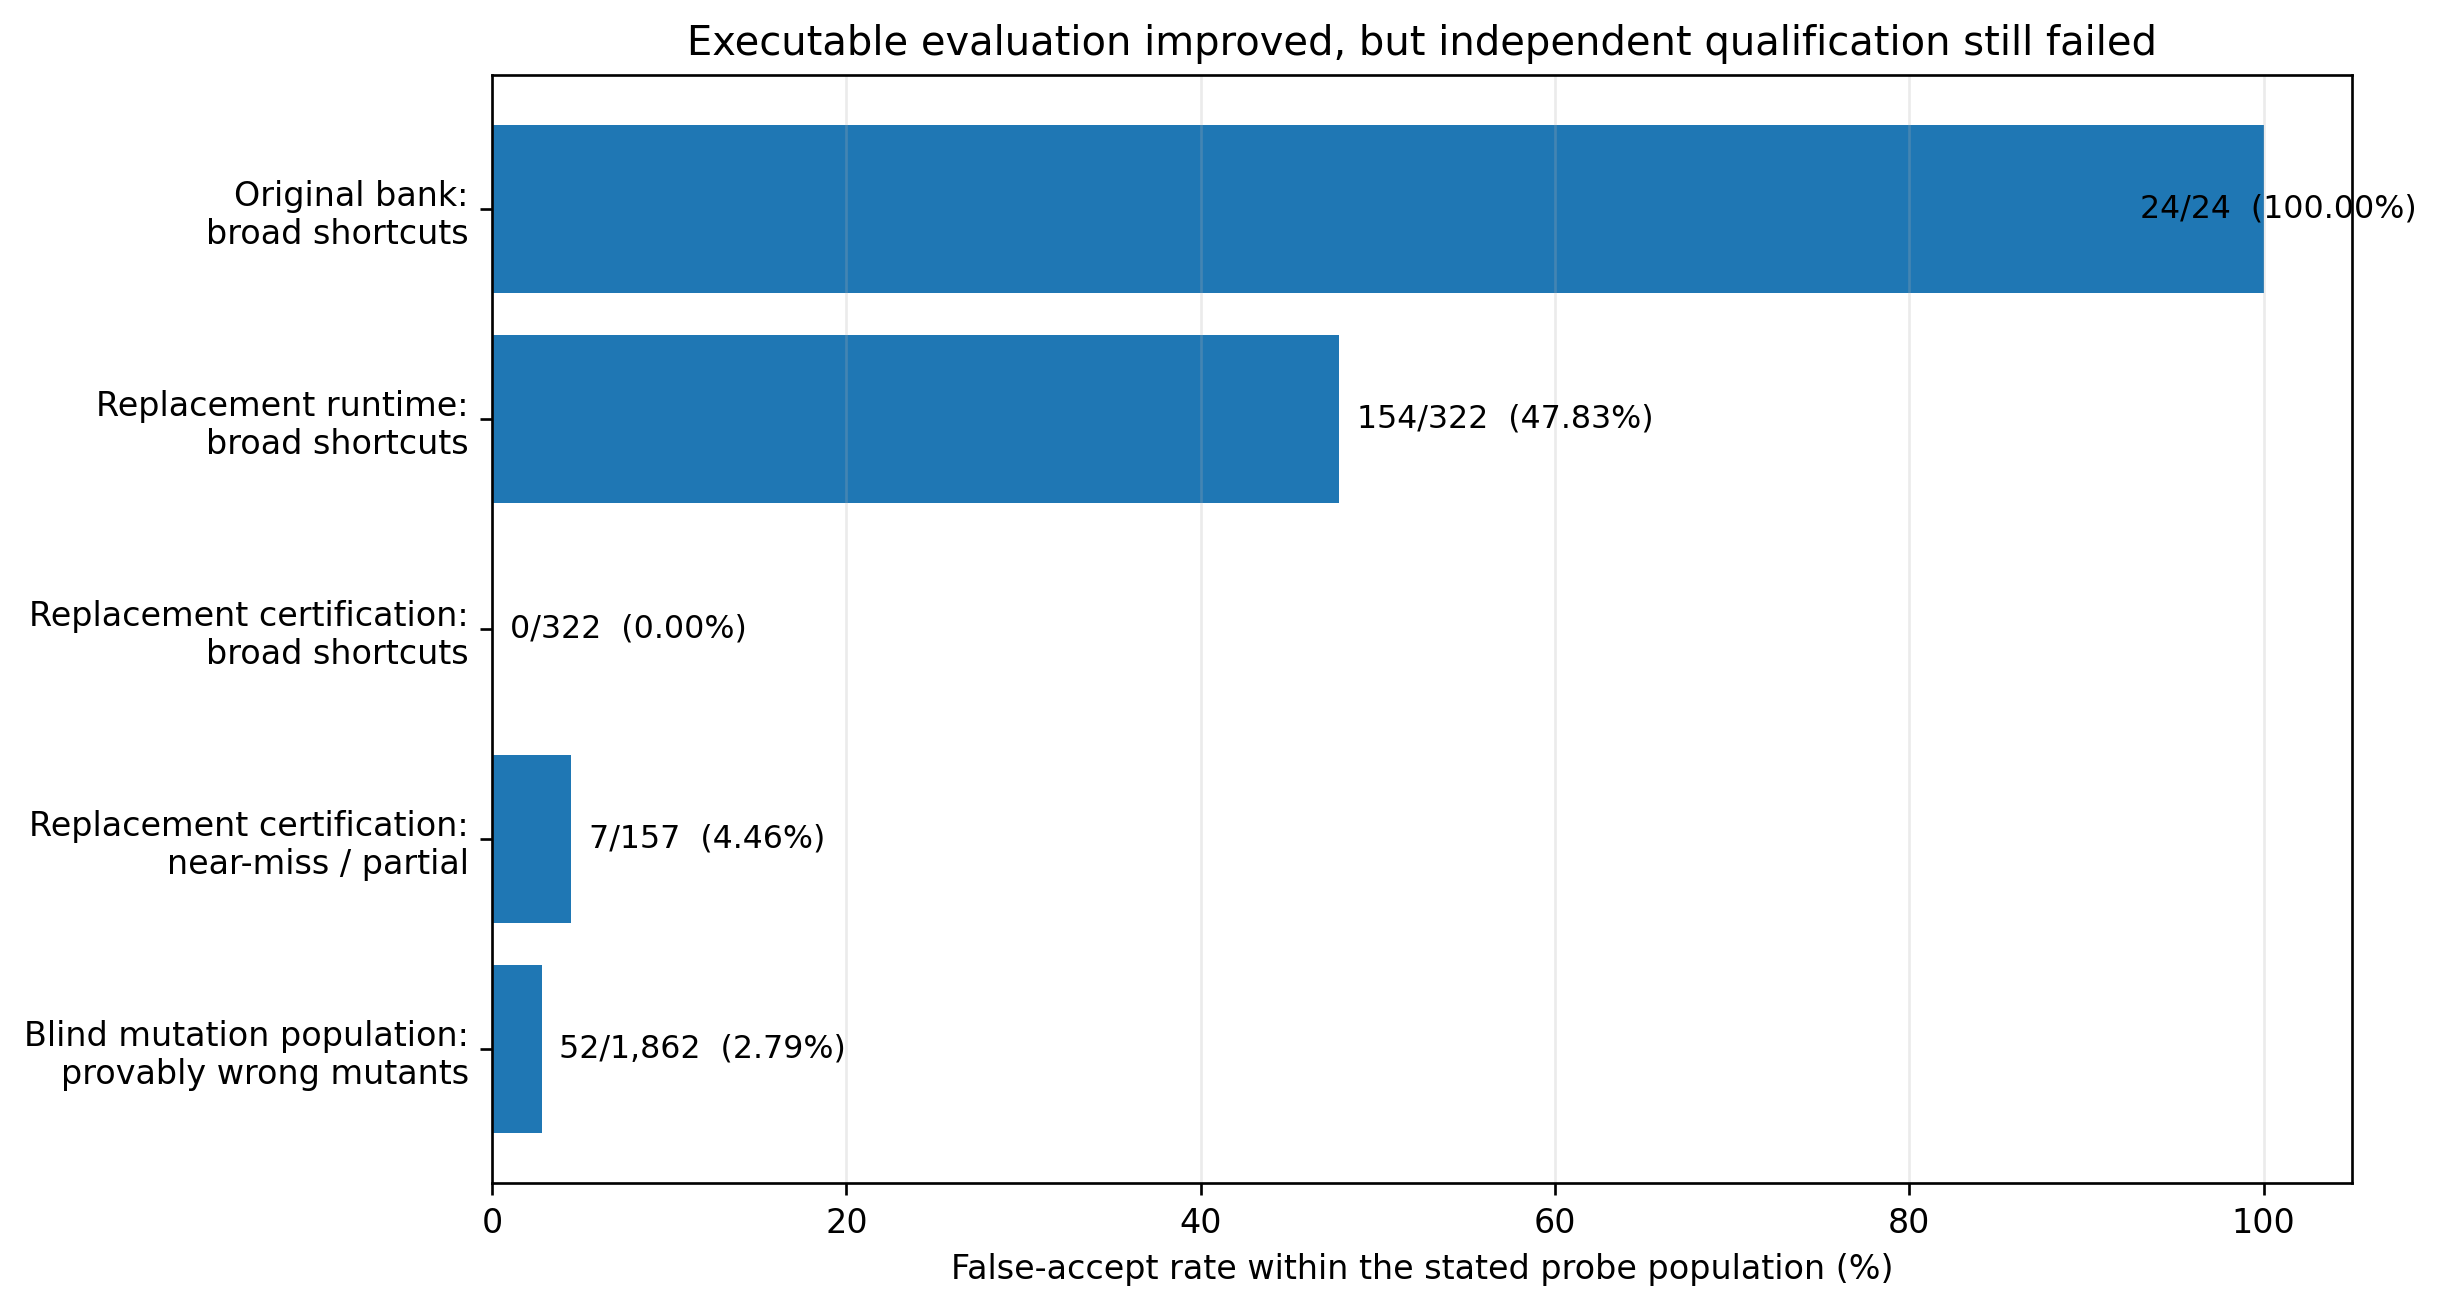
\includegraphics[keepaspectratio,alt={Figure 4. Evaluator qualification and failure surface. The replacement certification channel rejected broad shortcuts but still admitted near-miss programs and independently generated wrong mutants.}]{figures/figure4_evaluator_qualification.png}}

\subsubsection{4.8 The study repeatedly measured the wrong estimand
before correcting
it}\label{48-the-study-repeatedly-measured-the-wrong-estimand-before-correcting-it}

The evaluator defects were accompanied by statistical and data-retention
defects. They are not incidental implementation notes; each changed
which scientific sentence a number could support.

\paragraph{4.8.1 Cap exhaustion was excluded from the
denominator}\label{481-cap-exhaustion-was-excluded-from-the-denominator}

The first calibration scorer effectively estimated:

{[}
P(\textbackslash text\{correct\}\textbackslash mid\textbackslash text\{parseable
final\}) {]}

rather than the intended operational endpoint:

{[} P(\textbackslash text\{correct delivery\}) =
\textbackslash frac\{\textbackslash text\{correct final deliveries\}\}
\{\textbackslash text\{all model attempts\}\}. {]}

Episodes that exhausted their generation budget without a final answer
were labeled extraction failures and removed from the denominator. In
the retained calibration census, 88.5\% of logged extraction failures
were cap hits---the central phenomenon the study was intended to
measure.

After rewiring, the pooled reconciliation statistic moved from 0.9622 to
0.8386. That pooled figure is not itself a bank verdict because it
averages tasks selected for different strata and difficulty regimes. Its
purpose is to show that the two scorers answered materially different
questions.

The task-level consequence is simpler. A task with 25 correct finals and
five cap-exhausted attempts reads as 25/25 = 1.000 under the
parseable-final estimand and 25/30 = 0.833 under correct delivery. Under
the former, the task can be discarded as too easy. Under the latter, it
falls inside the intended difficulty band. The denominator therefore
changes bank membership, not merely a displayed percentage.

\paragraph{4.8.2 Medians were censored on the stratum that
mattered}\label{482-medians-were-censored-on-the-stratum-that-mattered}

In executable code, 55--64\% of episodes in several arms hit the
8,192-token cap. The observed median reasoning length was therefore
pinned at the censoring boundary. It was an unknown lower bound on the
true median, not a stable measure of central tendency.

The same episode records still supported two uncensored summaries:

\begin{itemize}
\tightlist
\item
  cap-exhaustion rate, which directly measures the censoring event; and
\item
  p25 reasoning length, which remained below the cap by construction.
\end{itemize}

Those quantities revealed the exploratory dose pattern in Table 2. The
correction did not justify selecting whichever statistic produced the
most favorable answer after results. It showed that the original primary
statistic could not measure its declared construct in the stratum where
censoring exceeded one half. A successor study must pre-register
censoring-aware endpoints before observing intervention outcomes.

\paragraph{4.8.3 Nominal task identifiers were not independent
experimental
units}\label{483-nominal-task-identifiers-were-not-independent-experimental-units}

The original code bank counted two decoding seeds within a task and ten
renamed clones within a family as though all task identifiers
contributed independent evidence. Correcting the unit from episode to
task changed one claimed significance result. Correcting it from nominal
task to semantic family widened the problem further.

The general rule adopted from this failure is:

\begin{quote}
The unit of analysis is the smallest unit that can vary independently
under the data-generating process, not the identifier emitted by the
evaluation harness.
\end{quote}

Seeds estimate within-task variation. They do not create new tasks.
Renamed copies estimate nothing about cross-problem generalization.

\paragraph{4.8.4 The analytical power calculation did not represent the
frozen decision
procedure}\label{484-the-analytical-power-calculation-did-not-represent-the-frozen-decision-procedure}

The planned CAP\_STRESS design used 18 tasks and 42 seeds per task and
was described as targeting 90\% power. A later simulator called the
actual conjunctive assessor rather than reproducing an isolated formula.
Under assumed discordance rates of 0.20, 0.35, and 0.50, realized power
at the frozen design was 0.816, 0.744, and 0.664, respectively---below
0.90 in every tested case.

The discrepancy had two sources. The analytical function was documented
as receiving between-task standard deviation while the test statistic
operated on observed per-task deltas, which also contain finite-seed
sampling variance. The actual gate additionally required bootstrap,
leave-one-task-out, breadth, and generator-family conditions omitted by
the formula. More seeds shrink within-task noise but do not remove
between-task heterogeneity.

These simulations still depended on assumed variance components, so they
are not a final power statement. Their valid contribution is
methodological: power must be simulated against the exact frozen
decision rule, using the same cluster structure and all conjunctive
gates. An analytic approximation to one component is an upper bound at
best.

\subsubsection{4.9 Reproducible artifacts selected the wrong authority
and exposed hidden
information}\label{49-reproducible-artifacts-selected-the-wrong-authority-and-exposed-hidden-information}

Content-addressed artifacts and extensive tests prevented several forms
of silent drift. They did not ensure that the production path used the
intended object.

One production calibration function booted the model and then selected
the parent P-BREVE-01 grading authority rather than the repaired R2
successor. The wave-rehearsal test did not catch the error because it
injected the correct authority directly into the scoring function. A
test that supplies the right dependency cannot discover that production
selects the wrong dependency. The execution could have produced
self-consistent records, complete hashes, and the wrong scientific
result.

The agentic harness had a separate information-flow defect.
\texttt{run\_tests()} returned one object containing captured standard
output and error. The harness persisted that object for the grader and
also serialized it into the model-visible conversation. On a failing
Python unit test, the payload could contain the hidden-test path, the
assertion source line, the expected literal, and the
actual-versus-expected difference. The grader and model needed different
channels; one shared object made hidden evidence part of the policy
context.

A successor scrubber separated a minimal model-facing result from the
full grader record and normalized hidden-path access attempts by intent
rather than exception type. Pre-scrub and post-scrub agentic results are
not directly comparable because the original model received materially
more information.

The frozen Python harness also carried a bytecode-cache hazard. A
same-length repair written and rerun within one wall-clock second could
execute stale \texttt{.pyc} code and be scored as still failing. A
tight-loop hardware reproduction produced false failures in 24 of 25
exposed trials under the frozen harness and 0 of 25 under the fixed
harness. That result must not be misread as the corruption rate of the
banked model run. Recovered reports showed 32 of 32 agentic episodes
passed, including all exposed reference-family cases; a false-negative
mechanism cannot have altered a run with zero observed failures. The
tight-loop result demonstrates reachability in replay or batch
regrading, not observed corruption of those episodes.

Finally, a protected-bank write path described as atomic validated all
changes before writing but applied the writes through a plain loop. An
exception after the second task could leave a partially mutated bank.
Verification atomicity is not write atomicity. The implementation had to
stage, validate, and commit one transaction rather than rely on an
all-or-nothing pre-check.

These cases share one lesson: artifact integrity describes the bytes
that were used or recorded. It does not establish that those bytes
represented the intended authority, estimand, information boundary, or
transaction.

\subsubsection{4.10 Final claim
disposition}\label{410-final-claim-disposition}

The study's final contribution is easier to understand by separating
retained measurements from interpretations that were withdrawn. The
labels below are publication dispositions, not replacements for the
claims-registry state machine.

{\def\LTcaptype{none} % do not increment counter
\begin{longtable}[]{@{}p{0.48\linewidth}p{0.46\linewidth}@{}}
\toprule\noalign{}
Report-local label & Meaning \\
\midrule\noalign{}
\endhead
\bottomrule\noalign{}
\endlastfoot
\textbf{Retained, narrowed} & The measurement or conclusion survives
after a named unsupported component is removed \\
\textbf{Not supported} & The frozen evidence did not satisfy the stated
hypothesis or threshold \\
\textbf{Withdrawn as an interpretation} & The underlying observation
remains historical evidence, but its causal or model-level reading is no
longer supportable \\
\textbf{Suspended} & The claim cannot be supported or refuted until it
is re-measured on a qualified instrument \\
\textbf{Contradicted} & Later evidence directly establishes that the
earlier statement is wrong \\
\textbf{Not measured} & The study did not collect evidence capable of
answering the question \\
\textbf{Rejected} & A release or portfolio disposition was affirmatively
denied \\
\end{longtable}
}

\textbf{Table 7. Claim disposition at the proposed report cutoff.}

{\def\LTcaptype{none} % do not increment counter
\begin{longtable}[]{@{}p{0.34\linewidth}p{0.28\linewidth}p{0.32\linewidth}@{}}
\toprule\noalign{}
Claim or interpretation & Final disposition & Reason \\
\midrule\noalign{}
\endhead
\bottomrule\noalign{}
\endlastfoot
The completed one-epoch full-recipe G4 result shows that the frozen
efficiency targets were not met & \textbf{Retained, narrowed
(\path{pbr2.g4.full-recipe-insufficient.015})} & The token and
termination components stand; the raw-code strict component is excluded
because the correctness bank was condemned \\
The configured one-epoch SFT+DPO recipe materially reduces reasoning &
\textbf{Not supported} & −10.9\% (longer) and +4.9\% (shorter) vs. a
+20\% two-seed target; DPO marginal effect approximately zero \\
A two-epoch DPO dose establishes a trained reasoning-efficiency benefit
& \textbf{Withdrawn as an interpretation} & The one-epoch null remains
unchanged; the apparent two-epoch effect was measured under
\texttt{xhigh}, and a neutral serving control reproduced it on untrained
weights \\
\texttt{medium} serving materially changes code-task termination
relative to \texttt{xhigh} on the screened shard & \textbf{Retained,
narrowed} & Observed cap hits 13/20 to 0/20 and RMST 6,407 to 608 on
untrained base; no broad correctness claim \\
The original executable-code bank measures functional correctness &
\textbf{Contradicted} & 24/24 broad adversarial non-solutions passed;
eight problems cloned tenfold; ambiguous residual tasks \\
The reported 0.844 fixed-policy correctness frontier is a product result
& \textbf{Suspended} & Correctness oracle condemned; relative verifier
error not shown to be arm-independent \\
The batch-2 runtime/certification bank is qualified & \textbf{Not
supported} & 7/157 near-miss/partial false accepts; 7/40 correct
references rejected by form; later AST audit derived 52 accepted mutants
from 1,862 provably wrong mutants \\
Cap exhaustion is an operational non-delivery phenotype &
\textbf{Retained, narrowed} & Directly observed termination outcome;
prevalence concentrated in selected tasks and not product-weighted \\
The model had already found an answer and then ``relitigated'' it &
\textbf{Not measured} & Requires trace-level or forced-final evidence
not collected here \\
The intervention preserved safety broadly & \textbf{Not measured} & Code
bank cannot measure refusal integrity, jailbreak resistance, or general
capability preservation \\
A model checkpoint is suitable for release & \textbf{Rejected} & Adapter
retired; no qualified bank, protected holdout, cross-domain promotion
gate, or external review \\
\end{longtable}
}

The result is not that nothing was learned. It is that the strongest
surviving findings concern the serving configuration and the evaluator,
not a successful trained model.

\subsection{5. Discussion}\label{5-discussion}

\subsubsection{5.1 The cheapest adequate control should precede weight
updates}\label{51-the-cheapest-adequate-control-should-precede-weight-updates}

P-BREVE began with a weight-level intervention because the target
behaviour appeared to require task-conditional reasoning allocation. The
serving-control result changes the order in which that hypothesis should
be tested.

On the screened code shard, a neutral \texttt{medium} setting removed
every observed cap hit from the untrained base and reduced restricted
mean reasoning length by roughly an order of magnitude. That does not
prove \texttt{medium} is globally optimal. Thinking-disabled serving
reduced token cost further and appeared directionally worse on
closed-form reasoning, although the clustered screen was too small to
establish that difference. Static low effort can also fail on tasks that
genuinely require depth.

The practical implication is not ``turn reasoning off.'' It is:

\begin{quote}
Before training a model to resist an effort instruction, compare it
against a controller that does not issue the instruction
indiscriminately.
\end{quote}

A future intervention should therefore evaluate at least three
matched-compute baselines:

\begin{enumerate}
\def\labelenumi{\arabic{enumi}.}
\tightlist
\item
  the stock or product-default serving policy;
\item
  a simple task-conditional controller over existing effort settings;
  and
\item
  the trained policy under the same controller and total compute budget.
\end{enumerate}

Only the third contrast identifies incremental weight-level value. If a
rule-based or learned controller captures most of the gain without
retraining each model family, it is likely to be easier to validate,
deploy, and transfer.

\subsubsection{5.2 Runtime success is a workflow signal, not a
correctness
certificate}\label{52-runtime-success-is-a-workflow-signal-not-a-correctness-certificate}

The replacement bank's runtime channel accepted 47.8\% of broad
shortcuts. This is not surprising and is not necessarily a defect in
runtime testing. A visible suite of three to five cases is meant to
provide fast feedback. It cannot remain secret from an agent that reads
and reruns it, and an optimizer can specialize to it.

The error is allowing the same signal to answer two questions:

\begin{itemize}
\tightlist
\item
  Should the system continue working on this attempt?
\item
  Is the completed artifact correct enough to support a scientific or
  production claim?
\end{itemize}

The first can use visible runtime feedback. The second requires an
independent certification channel. The certification channel must
contain cases that are not only different from runtime cases but
discriminating against programs that pass runtime for the wrong reason.

This distinction applies beyond coding. A cybersecurity repair can
satisfy a linter and violate the policy intent. An agent can reach a
desired final state through an unsafe transient state. A research
workflow can improve a public metric by exploiting data leakage. In each
case, a useful local signal becomes dangerous when promoted into final
authority.

\subsubsection{5.3 Coverage should be measured by killed alternatives,
not category
labels}\label{53-coverage-should-be-measured-by-killed-alternatives-not-category-labels}

Several failed certification sets contained many examples of the right
apparent category. They included empty inputs, ties, boundary-like
values, and malformed structures. Yet the wrong program still passed
because the examples did not separate its behaviour from the reference.

This is the difference between \textbf{shape coverage} and
\textbf{discrimination}. A test labeled ``empty input'' does not detect
every empty-input defect. A test containing a tie does not test the
declared tie-break unless two permitted outputs differ exactly on that
case. Two tests that separately exercise conditions A and B do not test
the conjunction A-and-B.

Mutation testing provides an operational measure: identify a program
that violates a stated requirement, find an input on which it differs,
and ask whether certification kills it. The mutation population must
include legitimate-alternative controls, because disagreement with one
reference is not equivalent to wrongness. It must also change after
repair, because a test suite built from one mutant family can overfit
that family.

\subsubsection{5.4 Evaluator qualification is part of the experiment,
not post hoc
hygiene}\label{54-evaluator-qualification-is-part-of-the-experiment-not-post-hoc-hygiene}

The original bank was evaluated after training. That order was
backwards. The study spent substantial compute and produced detailed
model comparisons before proving that its correctness authority rejected
trivial non-solutions or that its nominal tasks were independent.

The fact that the program later detected, documented, and corrected its
claims is valuable. It should not be used to pretend the initial process
was adequate. Several controls arrived only after the results they were
supposed to protect:

\begin{itemize}
\tightlist
\item
  semantic-family accounting followed clone-based analysis;
\item
  adversarial verifier qualification followed model evaluation;
\item
  denominator correction followed calibration;
\item
  censoring-aware endpoints followed a censored median;
\item
  production authority-selection testing followed implementation of a
  repaired loader; and
\item
  cluster-aware power simulation followed the frozen sample-size
  decision.
\end{itemize}

A stronger workflow qualifies the instrument before opening model
outcomes. At minimum, evaluator admission should be a separate gate with
its own failure budget and stop condition. A model experiment should not
be allowed to repair its evaluator indefinitely after observing which
tasks or metrics favor the intervention.

\subsubsection{5.5 A negative intervention result can still advance the
research
program}\label{55-a-negative-intervention-result-can-still-advance-the-research-program}

The configured recipe failed, the stronger adapter was retired, and no
release candidate emerged. Those facts do not make the work
unpublishable. They determine what the publication is about.

The report contributes a bounded result about one recipe and a more
general case study in evaluator validity. It shows how several
apparently reasonable practices fail in composition:

\begin{itemize}
\tightlist
\item
  running code is not the same as testing the specification;
\item
  hidden cases are not necessarily discriminating cases;
\item
  content addressing is not semantic validity;
\item
  repeated task identifiers are not independent evidence;
\item
  a smaller token count is not useful efficiency without verified
  delivery; and
\item
  a repair that kills known mutants is not proof that the defect class
  is closed.
\end{itemize}

Publishing the correction history also creates a stronger institutional
norm. A suspended claim should remain machine-readable as suspended. A
contradicted claim should not disappear from the ledger. A report should
distinguish a result that failed from a number that became
uninterpretable because its instrument failed.

\subsubsection{5.6 The durable research direction is verified adaptive
reasoning}\label{56-the-durable-research-direction-is-verified-adaptive-reasoning}

The model checkpoint is the least valuable artifact of this lineage. The
stronger direction is a system that allocates reasoning based on task
evidence while proving that reduced effort preserves the outcome that
matters.

That program requires three components:

\begin{enumerate}
\def\labelenumi{\arabic{enumi}.}
\tightlist
\item
  \textbf{A controller or intervention} that changes reasoning
  allocation.
\item
  \textbf{A qualified authority} that distinguishes correct delivery
  from shortcut compliance.
\item
  \textbf{A product-weighted measurement layer} that estimates how often
  the relevant phenomena occur outside an enriched mechanism bank.
\end{enumerate}

P-BREVE built fragments of all three and completed none at release
quality. The result nevertheless narrows the next experiment. Stronger
DPO on the same data and serving default is not the priority. Qualifying
the evaluator and establishing a controller baseline are.

\subsection{6. Limitations}\label{6-limitations}

\subsubsection{6.1 Development evidence, not
confirmation}\label{61-development-evidence-not-confirmation}

The report is based on internal development data and internally operated
infrastructure. No external laboratory reproduced the training or
evaluation. No external reviewer had custody of a primary holdout.
Several of the most important evaluator audits were initiated after the
original model results were visible. They support the diagnosis of the
instruments used; they do not turn the model experiment into a
pre-registered confirmatory study.

\subsubsection{6.2 One model lineage and one narrow intervention
family}\label{62-one-model-lineage-and-one-narrow-intervention-family}

The model evidence concerns one exact Qwen3.8-27B revision, one LoRA
target scope, one small SFT stage, one accepted DPO corpus, and a
bounded one-to-two-epoch dose range. It does not establish how
full-parameter training, online reinforcement learning, another
preference objective, another data mixture, or another model family
would behave.

The negative result is therefore configuration-specific. It is strong
enough to stop repeating the same recipe without a changed hypothesis.
It is not evidence that preference optimization cannot improve reasoning
efficiency in general.

\subsubsection{6.3 The original correctness evaluator was
invalid}\label{63-the-original-correctness-evaluator-was-invalid}

This is the report's central limitation and one of its main findings.
Any original semantic-success, strict-correctness, policy-ranking, or
capability-floor figure that depended on the condemned executable-code
bank is not a valid model result. The report retains such values only
where necessary to explain the correction history and labels them as
historical or suspended.

The evaluator failure also limits retrospective causal comparison. A
defective verifier does not necessarily bias every arm equally. Even
matched tasks do not make relative correctness safe when policies differ
in their propensity to emit shortcuts, alternate forms, or edge-case
errors.

\subsubsection{6.4 The serving-control screen was small and
clustered}\label{64-the-serving-control-screen-was-small-and-clustered}

The code-stratum serving comparison contained 20 episodes from ten
nominal tasks and two decoding seeds. Observing 0 of 20 cap hits at
\texttt{medium} does not establish a population cap rate of zero; the
exact two-sided 95\% upper bound remains substantial. The formal
matched-effort correctness comparison was underpowered and returned
\texttt{INDETERMINATE}.

The screen justifies retiring the adapter as an identified product
candidate because it exposes a dominant uncontrolled serving factor. It
does not prove that the adapter and base are behaviourally equivalent
under every task or metric.

\subsubsection{6.5 The banks were enriched and cannot estimate product
prevalence}\label{65-the-banks-were-enriched-and-cannot-estimate-product-prevalence}

Tasks were selected to expose reasoning-efficiency, cap-exhaustion,
discrimination, and verification phenomena. Such a bank is useful for
mechanism investigation and unsuitable for estimating how often ordinary
users encounter those phenomena.

The cap-stress pattern was also concentrated. In a later calibration
wave, 35 of 69 cap hits came from two tasks. Excluding those two, the
rate was approximately 6\% within that selected wave. Neither number
estimates product incidence. A product-impact claim requires a
separately sampled, product-weighted bank.

\subsubsection{6.6 Safety and broad capability were not measured
adequately}\label{66-safety-and-broad-capability-were-not-measured-adequately}

The replacement bank was executable code. It could measure code delivery
under its qualified portions and nothing broader. It did not measure
instruction following, mathematical reasoning outside the task set,
refusal integrity, jailbreak resistance, persona preservation, or
general agent safety.

This matters because length pressure can create failures outside code
correctness. A model may truncate a necessary refusal, answer less
often, omit qualifications, or skip tool verification. No statement in
this report should be read as evidence that those dimensions were
preserved.

The agentic harness leak additionally made pre-scrub safety comparisons
unclean. Model behaviour after seeing a hidden assertion cannot be
treated as behaviour under a protected evaluator.

\subsubsection{6.7 Cap exhaustion does not identify the internal
mechanism}\label{67-cap-exhaustion-does-not-identify-the-internal-mechanism}

A cap-exhausted episode proves that the model spent the available
generation budget and failed to deliver a final answer. It does not
prove that the model had already found the answer and then reconsidered
it. Establishing ``relitigation'' would require reasoning-trace
annotation, forced-final interventions, trajectory-prefix probes, or
stronger-policy comparisons that were not performed.

The report therefore uses operational language---budget exhaustion,
non-delivery, and termination---not a mechanistic claim about what the
model internally knew.

\subsubsection{6.8 Mutation populations were incomplete by
construction}\label{68-mutation-populations-were-incomplete-by-construction}

Human-designed shortcuts, witness-driven near misses, and first-order
AST mutations found different defects. None is exhaustive. AST mutation
does not reach every semantic error, stateful failure, multi-file
interaction, or alternative interpretation of the prompt. A low
false-accept rate against one population cannot be interpreted as a
general evaluator error rate.

The reported rates characterize the exact probe populations used. Their
strongest implication is qualitative: the bank failed a necessary
qualification test. They are not estimates of how frequently arbitrary
wrong programs would pass.

\subsubsection{6.9 Some calibration outputs could not be reconstructed
fully}\label{69-some-calibration-outputs-could-not-be-reconstructed-fully}

An early record format persisted a completion hash without retaining the
completion itself. As a result, some task identities for invalid
outputs, cap-versus-invalid decompositions, and per-task token summaries
could not be recovered. Later retention was changed to write
content-addressed completions before publishing scores. That repair
prevents recurrence and cannot reconstruct the missing historical
evidence.

The report excludes quantities that the surviving record cannot support.
The final evidence map should identify every figure derived from
complete retained outputs and every figure based on aggregate reports
only.

\subsubsection{6.10 Agent-assisted research is not independent
validation}\label{610-agent-assisted-research-is-not-independent-validation}

AI systems contributed substantially to implementation, adversarial
review, mutation generation, documentation, and analysis. Multiple model
families sometimes found different defects, which was useful. They also
repeated incorrect summaries, authored tests that passed for the wrong
reason, and propagated stale or reversed claims.

Model diversity is not equivalent to institutional independence. The
human author remains responsible for the protocol, claim boundaries,
corrections, and publication decision. An AI-generated review cannot be
cited as external peer review simply because it used a different model.

\subsection{7. Recommendations and Successor
Work}\label{7-recommendations-and-successor-work}

\subsubsection{7.1 Close the model intervention and separate evaluator
work}\label{71-close-the-model-intervention-and-separate-evaluator-work}

P-BREVE-01-R2 should close as a documented negative post-training result
with a linked evaluator-failure study. Continuing to repair the code
bank under the same open-ended lineage would prevent a stable report
cutoff and blur two different research questions:

\begin{enumerate}
\def\labelenumi{\arabic{enumi}.}
\tightlist
\item
  Did the SFT+DPO intervention work?
\item
  Can Vinci construct a trustworthy executable-code authority?
\end{enumerate}

The first has an answer at the present evidence tier: the configured
intervention did not establish a useful trained gain, and its apparent
stronger-dose effect was confounded by serving policy. The second
remains active research and should receive a separate program
identifier, charter, budget, and claims ledger.

\texttt{P-BREVE-02} should not be used for evaluator engineering. That
identifier is already reserved for a future locked-recipe reproduction
on a Western 24--32B base.

\subsubsection{7.2 Freeze a report cutoff rather than waiting for a
perfect
evaluator}\label{72-freeze-a-report-cutoff-rather-than-waiting-for-a-perfect-evaluator}

The report should bind to one repository commit and one evidence cutoff.
Findings after that point should enter an erratum only if they
invalidate a statement in this report; otherwise they belong to the
successor study.

Waiting until every evaluator problem is solved is not a scientific
requirement. It is a recipe for a paper that never closes. The report's
conclusion is partly that no qualified replacement instrument existed at
cutoff.

\subsubsection{7.3 Adopt Vinci Eval Integrity 0.1 before model
outcomes}\label{73-adopt-vinci-eval-integrity-01-before-model-outcomes}

The reusable output of the evaluator work is \textbf{Vinci Eval
Integrity 0.1}, a seven-check admission record for executable
evaluators. Version 0.1 is an internal, provisional standard derived
from failures measured in this program; it is not an external
certification. A bank may remain useful for development while one or
more checks are open, but it must not support model selection,
optimization, release, or product claims until all seven are evidenced.

\textbf{E1 --- Scope, identity, and statistical independence.} Every
task must bind a normalized prompt, signature, semantic-family
identifier, reference identity, and near-duplicate scan. Variants remain
within a cluster and are never counted as independent tasks. The
manifest must state the actual statistical unit rather than infer it
from task identifiers.

\textbf{E2 --- Contract clarity.} At least two implementers who have not
seen the reference or tests must implement the prompt independently and
pass certification. The prompt, not the reference implementation, is the
authority. Argument order, edge conditions, tie-breaks, state
transitions, and every behaviour tested by certification must be stated
or the task is rejected for repair.

\textbf{E3 --- Runtime/certification separation.} Visible runtime cases
may guide accept, retry, or repair decisions but may not determine the
scientific score. Protected certification must exercise behaviour absent
from runtime, remain unavailable to the policy context, and be loaded
through a separately identified channel. A runtime pass is explicitly
not a correctness certificate or an RL reward.

\textbf{E4 --- Bidirectional discrimination.} Certification must reject
broad shortcuts, plausible near misses, boundary and conjunction faults,
and independently generated mutations while accepting legitimate
alternative implementations. Qualification must include positive
controls expected to leak, negative controls expected not to leak, and
adjudication against the prompt contract rather than automatic deference
to the reference.

\textbf{E5 --- Estimand, censoring, and retention integrity.} Every
endpoint must define its denominator, censoring treatment, unit,
comparator, and direction before outcomes are opened. Cap exhaustion and
invalid delivery remain model outcomes rather than disappearing from the
denominator. Raw completions or sufficient non-lossy records must be
retained before scoring publishes, with schema versions preventing
incompatible resumes.

\textbf{E6 --- Production-path and authority binding.} Qualification
must exercise the actual loader, authority hash, environment, bytecode
policy, transaction semantics, hidden-information boundary, and
evidence-retention path used in production. Dependency injection of the
intended authority is not proof that production selects it. Protected
writes must be atomic, and model-visible tool output must be separated
from grader evidence.

\textbf{E7 --- Exact-procedure power and independent requalification.}
Power must be simulated against the complete frozen decision procedure
at the correct clustered unit, not against one convenient component.
After any repair, at least one fresh qualification population must be
constructed by a different method and by an origin independent of the
repair. A repair author cannot be the sole source of the population that
declares the repair complete.

Each check must emit a machine-readable artifact with a named owner,
status, evidence digest, and explicit failure condition. Passing seven
prose assertions is not passing the standard. Neither P-BREVE bank
cleared all seven checks at the proposed report cutoff.

\subsubsection{7.4 Make mutation qualification
bidirectional}\label{74-make-mutation-qualification-bidirectional}

A verifier must reject wrong programs and accept legitimate
alternatives. A test suite that kills every mutant by rejecting common
Python forms is not a correctness instrument.

Each qualification package should therefore contain:

\begin{itemize}
\tightlist
\item
  broad shortcuts;
\item
  plausible near-miss programs;
\item
  boundary and conjunction faults;
\item
  independently generated mutants;
\item
  multiple valid alternative implementations;
\item
  positive controls expected to leak;
\item
  negative controls expected to reject all mutants; and
\item
  adjudication based on the prompt contract rather than reference
  identity.
\end{itemize}

Repair authors must not generate the only population that validates
their repair. At least one post-repair population should be produced
through an independent construction method.

\subsubsection{7.5 Compare controllers before
retraining}\label{75-compare-controllers-before-retraining}

The next model experiment should begin with a serving-policy baseline. A
simple controller can use task features, confidence, tool state, elapsed
reasoning, or verifier feedback to select among \texttt{low},
\texttt{medium}, and higher effort. It should be evaluated at matched
total compute against:

\begin{itemize}
\tightlist
\item
  static \texttt{xhigh};
\item
  static \texttt{medium};
\item
  a simple rule-based controller;
\item
  a learned controller; and
\item
  the trained model under the same controller.
\end{itemize}

The trained-model contrast should answer whether weight updates add
value beyond a controller. A controller that reduces cost without
per-lineage retraining has a more favorable transfer and deployment
profile.

\subsubsection{7.6 Separate mechanism and product
banks}\label{76-separate-mechanism-and-product-banks}

A mechanism bank should be enriched for effort-responsive, cap-stress,
and verifier-challenging cases. A product bank should be sampled from
expected use. They should never be pooled into one headline percentage.

The mechanism bank answers why an intervention works or fails. The
product bank estimates user impact. A large effect on selected
cap-stress tasks can justify continued mechanism research and still have
negligible product prevalence.

\subsubsection{7.7 Add cross-domain promotion
gates}\label{77-add-cross-domain-promotion-gates}

No future P-BREVE checkpoint should become a product or release
candidate on code efficiency alone. Promotion should require separately
frozen checks for:

\begin{itemize}
\tightlist
\item
  executable-code correctness;
\item
  instruction following;
\item
  mathematical and general technical reasoning;
\item
  answer coverage and calibrated abstention;
\item
  refusal integrity and jailbreak resistance;
\item
  agentic tool-use correctness, including transient state; and
\item
  output-contract compliance.
\end{itemize}

The code mechanism bank can support a narrow research claim. It cannot
certify broad capability preservation or safety.

\subsubsection{7.8 Run P-BREVE-02 only after the instrument and
comparator are
fixed}\label{78-run-p-breve-02-only-after-the-instrument-and-comparator-are-fixed}

The reserved Western-base replication can be valuable, but only after
three preconditions are met:

\begin{enumerate}
\def\labelenumi{\arabic{enumi}.}
\tightlist
\item
  a qualified product and/or mechanism bank exists;
\item
  the serving controller is declared as a comparator before training;
  and
\item
  the intervention recipe is locked without access to the new model's
  protected outcomes.
\end{enumerate}

P-BREVE-02 should test transfer of a frozen method, not become another
recovery loop that changes data, dose, comparator, and evaluator after
each result.

\subsubsection{7.9 Publish the negative and corrective
artifacts}\label{79-publish-the-negative-and-corrective-artifacts}

Subject to licensing, privacy, and protection constraints, the public
package should include:

\begin{itemize}
\tightlist
\item
  the charter and amendments;
\item
  the exact model, tokenizer, template, adapter, and authority
  identities;
\item
  accepted-data manifests without restricted content where necessary;
\item
  training configuration and loss/mask audits;
\item
  raw oracle-independent episode summaries;
\item
  adversarial and mutation generators;
\item
  valid-alternative controls;
\item
  claim-ledger history, including suspended and contradicted records;
\item
  scripts that reproduce every public table; and
\item
  an explicit list of non-released protected artifacts.
\end{itemize}

The adapter itself should not be released as a model candidate.
Releasing the audit tooling and negative evidence is more scientifically
useful than distributing a checkpoint whose claimed benefit was not
established.

\subsection{8. Reproducibility and Evidence
Availability}\label{8-reproducibility-and-evidence-availability}

\subsubsection{8.1 Source identity}\label{81-source-identity}

\begin{itemize}
\tightlist
\item
  Research repository: \texttt{getsimpledirect/vinci-gpu-research}
  (private)
\item
  Program directory: \texttt{p-breve-01-r2/}
\item
  Technical-report repository:
  \texttt{getsimpledirect/vinci-technical-reports} (public)
\item
  Report evidence cutoff:
  \texttt{7cdfb4b68b7265be7f6c7299b107ff9d924f2a2d}
\item
  Published v1.0 source commit:
  \texttt{128dea8b4013cdb3398c98edab5dc930e24c51d2}, recorded by tag
  \texttt{tr3-v1.0.0}
\item
  Artifact digests: recorded in \texttt{CHECKSUMS.sha256} at the package
  root
\end{itemize}

Per-artifact evidence bindings, including the blob SHA of each
underlying record, are listed in \texttt{data/evidence\_bindings.json}.
The bound records reside in the private research repository; the commit
and blob SHAs identify them exactly and are verifiable by anyone granted
access to that repository.

\subsubsection{8.2 Recomputable
analyses}\label{82-recomputable-analyses}

The core evaluator analyses were run from the following private
implementations. Their evidence identities are fixed in
\texttt{data/evidence\_bindings.json}; the public aggregate values and
derivations distributed with this report are fixed in
\texttt{data/evaluator\_metrics.json},
\texttt{data/headline\_metrics.json}, and
\texttt{data/serving\_control.json}.

{\def\LTcaptype{none} % do not increment counter
\begin{longtable}[]{@{}p{0.34\linewidth}p{0.28\linewidth}p{0.32\linewidth}@{}}
\toprule\noalign{}
Analysis & Primary implementation & Required public output \\
\midrule\noalign{}
\endhead
\bottomrule\noalign{}
\endlastfoot
Original-bank adversarial audit & \texttt{scripts/verifier\_audit.py} &
probe definitions, aggregate JSON, rendered table \\
Batch-2 qualification & \texttt{scripts/verifier\_qualify\_b2.py} and
report renderer & all scored dispositions, exclusions, confidence
intervals \\
Blind mutation population &
\texttt{scripts/blind\_adversarial\_population.py} & mutation operators,
controls, per-task leaks, adjudication record \\
Serving-effort screen & \texttt{score\_effort\_screen.py} and frozen arm
manifests & episode identity, effort rendering proof, cluster-aware
summaries \\
Censoring and scorer reconciliation & \texttt{outcome\_scorer.py} and
calibration reports & old/new estimands, task-level worked example,
schema version \\
Cluster-aware power & \texttt{scripts/cluster\_aware\_power.py} &
simulation configuration, seed, intervals, exact frozen assessor
identity \\
Claims reconciliation & \texttt{claims.jsonl} plus registry validator &
complete tier history and supersession map \\
\end{longtable}
}

The original verifier audit was run with explicit zero-tolerance
thresholds rather than hidden defaults. The batch-2 qualification
similarly recorded the exact frozen authority hashes on every run. For
this repository-forward candidate, the package inventory binds the
distributed evidence records and rendered surfaces by SHA-256; the
private-record commit and blob identities remain independently listed in
\texttt{data/evidence\_bindings.json}.

\subsubsection{8.3 Protected and unavailable
materials}\label{83-protected-and-unavailable-materials}

Not every artifact can or should be public.

\begin{itemize}
\tightlist
\item
  Protected certification cases must remain unavailable to any policy
  that may later be scored against them.
\item
  Credentials, internal infrastructure configuration, and private
  artifact locations must be removed.
\item
  Training examples inherited under restricted or unclear redistribution
  terms must be represented by hashes and provenance rather than
  republished.
\item
  Missing historical completions cannot be reconstructed from their
  hashes and should be listed as unavailable.
\item
  The retired adapters may be archived internally for evidence identity
  without being promoted as downloadable models.
\end{itemize}

A reproducibility statement should distinguish \textbf{computational
reproduction of the published tables} from \textbf{independent
replication on a fresh protected bank}. The former may be possible from
released summaries and probes. The latter was not completed in this
study.

\subsubsection{8.4 Publication manifest
standard}\label{84-publication-manifest-standard}

At report cutoff, the program adopted the following archival-manifest
standard. The public package records its distributed-file inventory in
\texttt{MANIFEST.json} and \texttt{CHECKSUMS.sha256}; restricted
research identities remain in the evidence register described in Section
8.1.

\begin{itemize}
\tightlist
\item
  report title, version, date, and series number;
\item
  sole-author identity and contribution approval commit;
\item
  source commit and clean-tree proof;
\item
  report Markdown, LaTeX, HTML, DOCX, and PDF hashes, if those formats
  are generated;
\item
  every figure source and hash;
\item
  every table's source artifact and derivation command;
\item
  every signed metric's canonical name, formula, unit, comparator,
  positive direction, and zero interpretation;
\item
  model, tokenizer, template, and serving-stack identities;
\item
  checkpoint tree hashes with the hash algorithm named explicitly;
\item
  authority and evaluator identities;
\item
  claims-registry snapshot;
\item
  known exclusions and non-public artifacts; and
\item
  external-review status.
\end{itemize}

Hash values without their algorithms are insufficient. This program
produced a false checkpoint-mutation alarm by comparing two valid but
algorithmically different tree digests over the same bytes.

\subsection{9. Conclusion}\label{9-conclusion}

P-BREVE-01-R2 did not produce a successful reasoning-efficiency model.
The configured one-epoch SFT-to-DPO recipe missed its reasoning and
generation targets at both fixed seeds, and the marginal DPO effect over
SFT was approximately zero. A stronger DPO dose appeared to improve
code-task termination under the study's \texttt{xhigh} serving
condition, but a neutral \texttt{medium} setting reproduced nearly the
entire termination change on untrained base weights. The adapter was
retired and no checkpoint was selected for release.

The more consequential result was that the evaluator could not support
the apparent correctness story. The original code bank accepted every
broad adversarial shortcut tested, counted eight repeated problems as 80
tasks, and turned ambiguous specifications into apparent capability
failures. A replacement runtime/certification design rejected broad
shortcuts much more effectively, yet still accepted near-miss programs
and rejected correct references for non-behavioural reasons. The blind
AST population found leaks in 19 of 40 tasks; combining the original
seven-task witness set with the fourteen newly adjudicated tasks outside
it yielded a cross-method known-flaw lower bound of at least 21 of 40.

The study therefore supports a different research conclusion from the
one it began seeking:

\begin{quote}
Efficient reasoning is not established by producing fewer tokens or by
passing executable checks. It is established only when reduced
computation preserves delivery under an evaluator that has itself
survived independent attempts to make wrong work look correct.
\end{quote}

This is a negative intervention result, not a null research result. It
redirects the next program toward controller-first baselines, evaluator
admission before model training, semantic-family-aware statistics,
censoring-aware endpoints, and strict separation between runtime
feedback and certification authority.

No model, evaluator bank, or product claim from P-BREVE-01-R2 is
recommended for release. The report was selected as the
program\textquotesingle s sole public release artifact.

\subsection{Author Contributions}\label{author-contributions}

George Pu is the sole scholarly author.

\textbf{George Pu:} conceptualization, methodology, investigation,
formal analysis, validation, data curation oversight, supervision,
project administration, visualization, claim governance, and
writing---original draft and review and editing. George served as
decision owner for the program and accepts responsibility for the
protocol decisions, interpretation, corrections, and publication claims.

AI-system assistance and non-author contributions are disclosed below
and do not constitute scholarly authorship.

\subsection{Competing Interests, Funding, and AI
Assistance}\label{competing-interests-funding-and-ai-assistance}

George Pu is the founder of SimpleDirect / Vinci Research, which
designed and operated P-BREVE. The study evaluated internally developed
training and evaluation infrastructure and could affect Vinci's research
positioning. No model checkpoint from the study is being marketed or
recommended for deployment.

The study used company-controlled compute, funded by SimpleDirect.

No external funding was received for the work reported here, and no
funder had any role in study design, analysis, interpretation, or the
decision to publish.

No external peer review or independent external audit was performed for
the report cutoff.

AI systems from OpenAI and Anthropic assisted with software
implementation, research planning, data and artifact checks, adversarial
review, mutation generation, analysis packaging, documentation,
consistency review, and manuscript drafting. AI-generated outputs were
treated as proposals or evidence-processing assistance, not as scholarly
authorship or independent validation. The human author remains
responsible for protocol decisions, factual verification, corrections,
interpretation, and publication claims.

\subsection{Ethics and Safety
Statement}\label{ethics-and-safety-statement}

The study involved no human subjects and did not collect personal data
for the reported analyses. It evaluated open-weight language-model
behaviour on internally constructed technical tasks. Protected evaluator
cases are withheld to preserve measurement integrity. The report does
not release a trained checkpoint or an executable reward bank because
neither met the program's release standard.

The adversarial programs described here were designed to test
correctness evaluators in a controlled code sandbox. They are ordinary
task-specific shortcuts, not malware, and the report omits
infrastructure credentials and private operational details.

\subsection{References}\label{references}

{[}1{]} Qwen Team. ``Qwen3.8.'' Official model release and model
documentation, August 2026. Model identifier used in this study:
\texttt{Qwen/Qwen3.8-27B}.

{[}2{]} Rafael Rafailov, Archit Sharma, Eric Mitchell, Stefano Ermon,
Christopher D. Manning, and Chelsea Finn. ``Direct Preference
Optimization: Your Language Model Is Secretly a Reward Model.''
\emph{Advances in Neural Information Processing Systems}, 2023.
arXiv:2305.18290.

{[}3{]} Xiang Liu, Xuming Hu, Xiaowen Chu, and Eunsol Choi. ``DiffAdapt:
Difficulty-Adaptive Reasoning for Token-Efficient LLM Inference.''
arXiv:2510.19669, 2025.

{[}4{]} Junda Wang, Zhichao Yang, Dongxu Zhang, Sanjit Singh Batra, and
Robert E. Tillman. ``ESTAR: Early-Stopping Token-Aware Reasoning for
Efficient Inference.'' arXiv:2602.10004, 2026.

{[}5{]} Mohammed Ehab, Aymane El Gadarri, Vivek F. Farias, Adam
Jozefiak, and Ciamac C. Moallemi. ``OS-Pruner: Pruning Chains-of-Thought
of Reasoning Models via Optimal Stopping.'' arXiv:2607.11089, 2026.

{[}6{]} Jingbo Yang, Bairu Hou, Wei Wei, Yujia Bao, and Shiyu Chang.
``Ares: Adaptive Reasoning Effort Selection for Efficient LLM Agents.''
arXiv:2603.07915, 2026.

{[}7{]} Yiwen Zhang, Xiaodong Yan, Zhenyu Huang, Deng Zhao, Liang Jiang,
Qing Cui, Zujie Wen, Zhiqiang Zhang, and Jun Zhou. ``Robust Code RL via
Faulty-Code-Driven Test Case Synthesis and Dense Reward Shaping.''
arXiv:2608.24135, 2026.

{[}8{]} Yuxuan Sun, Yuze Zhao, Yufeng Wang, Yao Du, Zhiyuan Ma, Jinbo
Wang, Mengdi Zhang, Kai Zhang, and Zhenya Huang. ``SWE-Mutation: Can
LLMs Generate Reliable Test Suites in Software Engineering?''
arXiv:2605.22175, 2026.

{[}9{]} Shahbaz Siddeeq, Muhammad Waseem, Umar Subhan Malhi, and Pekka
Abrahamsson. ``CodeAssay: A Multi-Metric Benchmark with Audited Ground
Truth for LLM Code Generation.'' arXiv:2608.03535, 2026.

{[}10{]} Pradyumna Shyama Prasad, Meiri Anto, Leon Eshuijs, Julian
Moncarz, Kaustubh Kislay, and Juan J. Vazquez. ``BAITBENCH: Measuring
Agent Reward Hacking with Optional Shortcuts Planted in ML Tasks.''
arXiv:2608.30724, 2026.

{[}11{]} Yue Jia and Mark Harman. ``An Analysis and Survey of the
Development of Mutation Testing.'' \emph{IEEE Transactions on Software
Engineering} 37, no. 5 (2011): 649--678.
\url{https://doi.org/10.1109/TSE.2010.62}.

\subsection{Appendix A. Claim-to-Evidence
Boundary}\label{appendix-a-claim-to-evidence-boundary}

\pandocbounded{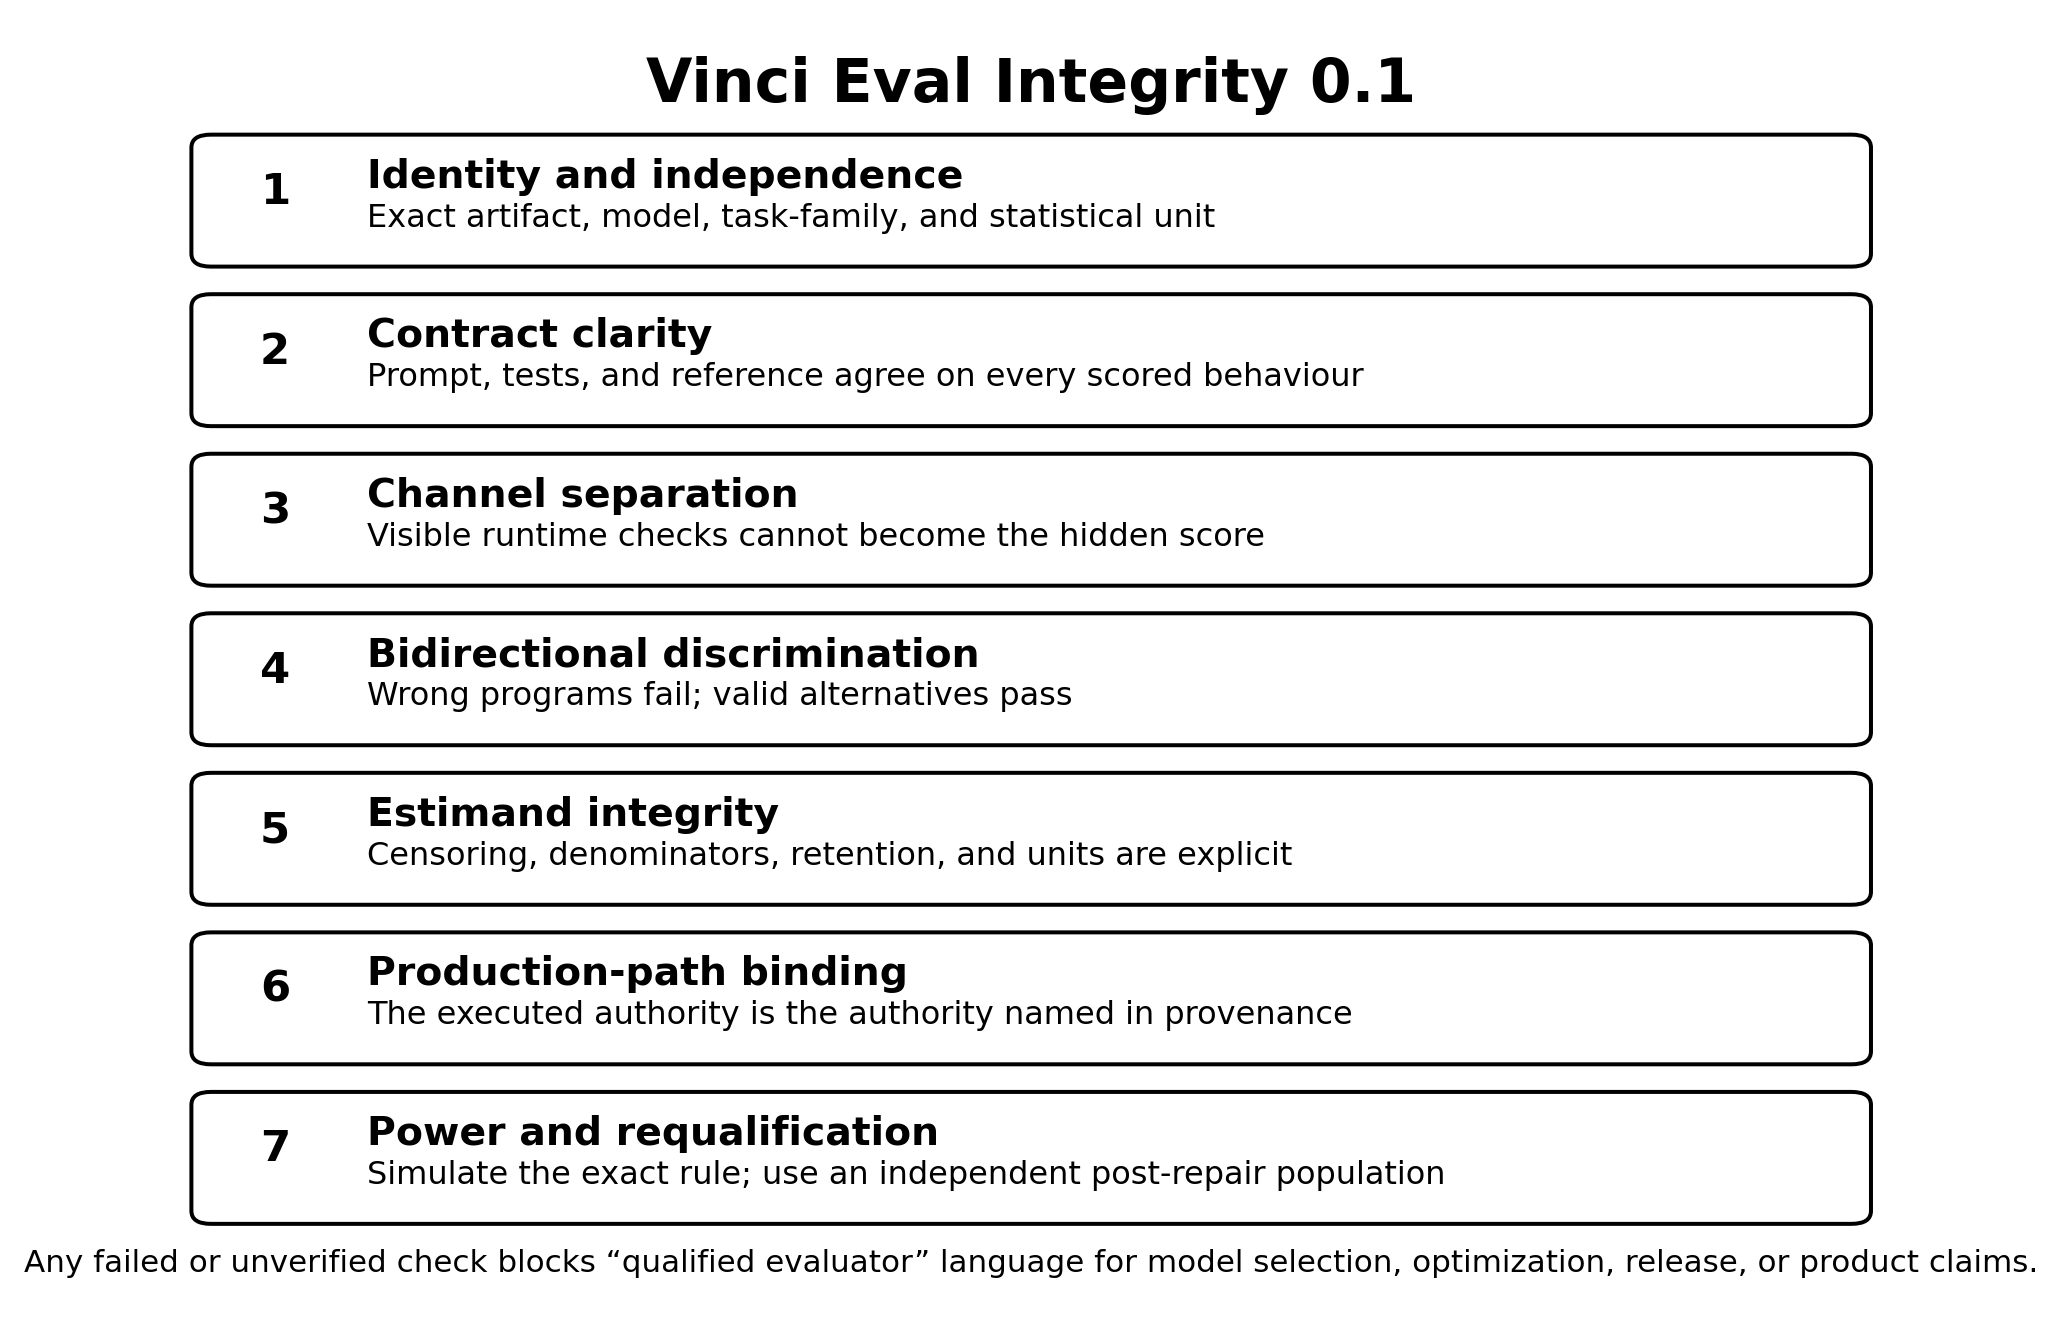
\includegraphics[keepaspectratio,alt={Figure 6. Vinci Eval Integrity 0.1. Seven checks convert the study's evaluator failures into a reusable admission record.}]{figures/figure6_vinci_eval_integrity.png}}

This appendix is the final human-readable claim-to-evidence boundary for
the v1.0 analysis. The ``public sentence'' column is deliberately
narrower than the underlying internal record, and the distributed claim
dispositions are machine-readable in
\texttt{data/claim\_dispositions.json}.

\subsubsection{A.1 Derived-quantity
register}\label{a1-derived-quantity-register}

A source hash proves which bytes were read; it does not by itself define
how adjacent fields were assembled into a report-level ratio or union.
The package records the following derivations directly in
\texttt{data/evaluator\_metrics.json}; this table is their report
rendering.

{\def\LTcaptype{none} % do not increment counter
\begin{longtable}[]{@{}p{0.28\linewidth}p{0.25\linewidth}p{0.21\linewidth}p{0.20\linewidth}@{}}
\toprule\noalign{}
Report rendering & Source fields & Deterministic derivation & Required
qualifier \\
\midrule\noalign{}
\endhead
\bottomrule\noalign{}
\endlastfoot
\texttt{154/322} broad shortcuts pass runtime &
\texttt{runtime\ shortcuts\ that\ pass\ =\ 154}; broad-shortcut
population \texttt{=\ 322} & \texttt{154\ ÷\ 322} & runtime channel;
families 1--5 \\
\texttt{7/157} near-miss/partial programs pass certification & near-miss
\texttt{4/121}; partial \texttt{3/36} &
\texttt{(4\ +\ 3)\ ÷\ (121\ +\ 36)} & certification channel; designed
probe population \\
\texttt{52/1,862} blind mutants pass certification & protected-bank
\texttt{accepted\ by\ certification\ =\ 52};
\texttt{provably-wrong\ mutants\ =\ 1,862} & \texttt{52\ ÷\ 1,862} &
first-order AST population \\
\texttt{19/40} AST-leak tasks & \texttt{tasks\ with\ a\ leak\ =\ 19};
protected tasks \texttt{=\ 40} & \texttt{19\ ÷\ 40} & detected by the
AST population \\
\texttt{21/40} AST-no-leak tasks & protected tasks \texttt{=\ 40};
AST-leak tasks \texttt{=\ 19} & \texttt{(40\ −\ 19)\ ÷\ 40} & \textbf{no
leak detected by this population} \\
\texttt{at\ least\ 21/40} cross-method known-flaw union & previously
identified witness tasks \texttt{=\ 7}; newly adjudicated tasks outside
that set \texttt{=\ 14} & \texttt{(7\ +\ 14)\ ÷\ 40} & \textbf{known
flaw under at least one method; lower bound} \\
\end{longtable}
}

The two \texttt{21/40} renderings have opposite polarity and must never
be cited without their qualifier.

\subsubsection{A.2 Public claim
boundary}\label{a2-public-claim-boundary}

{\def\LTcaptype{none} % do not increment counter
\begin{longtable}[]{@{}p{0.28\linewidth}p{0.25\linewidth}p{0.21\linewidth}p{0.20\linewidth}@{}}
\toprule\noalign{}
Public sentence & Evidence class & Supporting artifact family &
Prohibited expansion \\
\midrule\noalign{}
\endhead
\bottomrule\noalign{}
\endlastfoot
The configured one-epoch recipe missed the frozen efficiency targets &
Oracle-independent token summaries, two fixed seeds & claim
\texttt{.015}, final G4 arm reports, and final decision packet & ``DPO
cannot improve reasoning efficiency'' \\
One-epoch DPO added approximately zero median-reasoning change over SFT
& Matched arm token summaries & SFT-only and final-adapter reports &
``The adapters are behaviourally identical'' \\
Under \texttt{xhigh}, a two-epoch dose reduced code p25 and cap
exhaustion & Exploratory token and termination summaries & dose-response
arm reports & ``The dose produced a useful model'' \\
Base@\texttt{medium} changed observed code termination relative to
base@\texttt{xhigh} & Shared-shard serving screen & six-arm
effort-screen reports & ``Medium has a true zero cap rate'' or ``medium
is globally optimal'' \\
The original code bank was not a valid correctness instrument &
Executable adversarial audit & verifier adequacy JSON and probe code &
``The model reward-hacked the bank'' \\
The 80 nominal code tasks represented eight repeated problems &
Structural content comparison & family/clone audit & a universal 3.16
correction for other banks \\
Batch-2 certification rejected all 322 broad shortcuts & Qualification
probe population & batch-2 audit summary & ``The certification bank is
qualified'' \\
Batch-2 certification accepted 7 of 157 near-miss/partial programs &
Qualification probe population & batch-2 audit summary; derivation
\texttt{(4\ +\ 3)/(121\ +\ 36)} & a deployment false-accept rate \\
The frozen authority rejected 7 of 40 correct references & Reference
execution and AST-path audit & batch-2 audit and corrected claim
\texttt{.014} & ``17.5\% of model-generated correct programs are
rejected'' \\
Blind mutation found 52 of 1,862 provably wrong mutants passing across
19 of 40 protected tasks & First-order AST mutation population &
protected-bank cells \texttt{52} and \texttt{1,862}, task count
\texttt{19/40}, source blob
\texttt{1bb4ea390b38eb4f90d1519933b4e850ede93065}, and underlying audit
artifact & an exhaustive defect count or deployment false-accept rate \\
At least 21 of 40 tasks had a known certification flaw & Union of two
non-exhaustive methods & seven previously identified Defect-B tasks plus
fourteen newly adjudicated tasks outside that set & the distinct
\texttt{21/40} AST-no-leak count, or an estimate that exactly 52.5\% of
tasks are defective \\
The original 0.844 correctness frontier is suspended & Claims registry
and condemned instrument & claim \texttt{.010} & any current product
ranking \\
No checkpoint is recommended for release & Program disposition &
roadmap, status, claims registry & ``The base model is unsafe'' or ``the
method can never work'' \\
\end{longtable}
}

\subsection{Appendix B. Correction and Withdrawal
Timeline}\label{appendix-b-correction-and-withdrawal-timeline}

{\def\LTcaptype{none} % do not increment counter
\begin{longtable}[]{@{}p{0.34\linewidth}p{0.28\linewidth}p{0.32\linewidth}@{}}
\toprule\noalign{}
Date, 2026 & Event & Claim consequence \\
\midrule\noalign{}
\endhead
\bottomrule\noalign{}
\endlastfoot
17 August & R2 recovery charter and data/training program authorized &
P-BREVE-01 negative result preserved; R2 begins \\
17--18 August & Data acceptance, SFT, DPO, and two-seed G4 execution &
One-epoch recipe reaches final decision surface \\
18 August & One-epoch decision packet reports failed efficiency target
and approximately zero DPO marginal effect & Negative configured-recipe
result established \\
18--19 August & Bounded two-epoch dose screen & Apparent code-stratum
dose response under \texttt{xhigh} \\
19 August & Native effort screen varies serving controls & Trained
interpretation becomes unresolved; controller hypothesis elevated \\
19--20 August & Original-bank adversarial audit & Correctness figures
withdrawn; policy frontier suspended; RL prohibition imposed \\
20 August & Replacement-bank qualification audit & Runtime/certification
split shown non-redundant; near-miss and AST false-rejection defects
found \\
20 August & A claim records the seven-reference result in the wrong
direction & Claim marked contradicted and superseded by corrected
\texttt{.014} \\
20--21 August & Denominator, calibration-arm, retention, confidence, and
power corrections & Several apparent bank-membership and power
statements withdrawn or narrowed \\
21--23 August & Targeted repairs and fresh blind mutation populations &
Repairs fail to generalize; protected bank remains unqualified \\
23--26 August & Production-path, write-atomicity, bytecode, and
authority-wiring audits & Reproducibility package strengthened; no model
claim restored \\
Report cutoff & Model intervention closed; evaluator work separated & No
model, bank, or release candidate \\
\end{longtable}
}

This chronology intentionally remains day-level context rather than a
commit ledger. Exact identities for the report source, evidence cutoff,
underlying evidence blobs, and distributed artifacts are recorded in
Section 8.1, \texttt{data/evidence\_bindings.json},
\texttt{MANIFEST.json}, and \texttt{CHECKSUMS.sha256}.

\subsection{Appendix C. Vinci Eval Integrity 0.1 --- Seven-Check
Admission
Record}\label{appendix-c-vinci-eval-integrity-01--seven-check-admission-record}

Vinci Eval Integrity 0.1 packages the program's evaluator lessons into a
reusable admission record. Each row must carry \texttt{status},
\texttt{owner}, \texttt{evidence\_digest}, \texttt{failure\_condition},
and \texttt{last\_verified}. The standard is conjunctive: one failed or
unverified row prevents a bank from being called qualified for
model-selection, optimization, release, or product claims.

{\def\LTcaptype{none} % do not increment counter
\begin{longtable}[]{@{}p{0.28\linewidth}p{0.25\linewidth}p{0.21\linewidth}p{0.20\linewidth}@{}}
\toprule\noalign{}
ID & Check & Minimum sealed evidence & Fail condition \\
\midrule\noalign{}
\endhead
\bottomrule\noalign{}
\endlastfoot
\textbf{E1} & Scope, identity, and independence & Normalized prompt and
signature; semantic-family ID; reference identity; pairwise
duplicate/near-duplicate scan; declared cluster unit & Nominal IDs
substitute for independent problems, or the analysis unit is not
declared \\
\textbf{E2} & Contract clarity & Two prompt-only blind implementations;
certification outcomes; explicit argument order, edge cases, tie-breaks,
and state semantics & A competent independent implementation fails
because the prompt leaves a tested behaviour unstated \\
\textbf{E3} & Runtime/certification separation & Distinct files,
digests, loaders, and access controls; documented novel-behaviour
coverage; runtime-purpose statement & Policy can access certification,
channels collapse, or runtime pass is used as the final score/reward \\
\textbf{E4} & Bidirectional discrimination & Broad shortcuts; near
misses; boundary/conjunction faults; independent mutations; valid
alternatives; positive and negative controls; prompt-based adjudication
& A provably wrong program certifies, a valid alternative is rejected
without behavioural cause, or controls cannot distinguish leak/no-leak
states \\
\textbf{E5} & Estimand, censoring, and retention & Endpoint formula,
unit, denominator, comparator, direction, censoring rule, raw-completion
retention, schema version & Cap/invalid outcomes disappear, the sign is
ambiguous, or the published number cannot be reconstructed at the
required unit \\
\textbf{E6} & Production-path and authority binding & End-to-end
rehearsal of actual loader, authority hash, environment, bytecode
policy, atomic write path, hidden-information boundary, and evidence
sink & Qualification supplies the right authority rather than proving
production selects it, writes can partially commit, or grader-only data
reaches the model \\
\textbf{E7} & Exact-procedure power and independent requalification &
Cluster-aware simulation against the full frozen assessor; simulation
uncertainty; fresh post-repair population from a different construction
method and origin & Power is inferred from a component formula, seeds
are counted as tasks, or the repair population validates its own
patch \\
\end{longtable}
}

The detailed implementation checklist may evolve under later versions,
but these seven checks should remain separately reportable. Combining
them into a single ``evaluation passed'' flag would recreate the
compression error this report documents.

\subsection{Appendix D. Proposed Figures and
Tables}\label{appendix-d-proposed-figures-and-tables}

This appendix records the specification for each figure and table. The
six figures specified here were generated from the frozen result set by
\texttt{source/build\_figures.py} and appear in the body of this report.

\subsubsection{Figure 1 --- Study lineage and claim
disposition}\label{figure-1--study-lineage-and-claim-disposition}

A left-to-right state diagram:

\texttt{P-BREVE-01\ no-go} → \texttt{R2\ data/SFT/DPO} →
\texttt{one-epoch\ negative} → \texttt{two-epoch\ apparent\ dose} →
\texttt{serving-control\ confound} →
\texttt{original-bank\ condemnation} →
\texttt{replacement-bank\ qualification\ failure} →
\texttt{no\ release}.

Show \texttt{P-BREVE-02} as a separate reserved future branch, not the
endpoint of R2.

\subsubsection{Figure 2 --- Experimental and audit
design}\label{figure-2--experimental-and-audit-design}

Two layers:

\begin{itemize}
\tightlist
\item
  model layer: base, SFT, DPO-1, DPO-2 crossed with fixed seeds and
  effort controls;
\item
  authority layer: runtime tests, certification tests, broad probes,
  near-miss probes, valid alternatives, and blind mutations.
\end{itemize}

\subsubsection{Figure 3 --- Serving control on executable
code}\label{figure-3--serving-control-on-executable-code}

Use two separate panels or figures rather than dual axes:

\begin{itemize}
\tightlist
\item
  observed cap-hit count out of 20;
\item
  RMST reasoning tokens.
\end{itemize}

Display confidence intervals or the observed denominators. Do not plot
0/20 as an exact zero without uncertainty.

\subsubsection{Figure 4 --- Verifier qualification
funnel}\label{figure-4--verifier-qualification-funnel}

Show:

\begin{itemize}
\tightlist
\item
  original bank: 24/24 broad attacks accepted;
\item
  batch 2: 0/322 broad attacks accepted at certification;
\item
  batch 2: 7/157 near-miss/partial attacks accepted, derived as
  \texttt{(4\ +\ 3)/(121\ +\ 36)};
\item
  blind protected audit: 52/1,862 mutants accepted across 19/40 AST-leak
  tasks, derived from adjacent protected-bank cells in
  \path{p-breve-01-r2/docs/BLIND-ADVERSARIAL-POPULATION.md};
\item
  cross-method known-flaw union: seven previously identified tasks plus
  fourteen newly adjudicated outside that set, yielding at least 21/40;
\item
  source-document complement, shown only as a warning label if included:
  21/40 AST-no-leak tasks = \texttt{40\ −\ 19}, which has the opposite
  polarity.
\end{itemize}

\subsubsection{Figure 5 --- Final claim
boundary}\label{figure-5--final-claim-boundary}

Three columns:

\begin{itemize}
\tightlist
\item
  \textbf{Retained:} one-epoch token null, cap/termination observations,
  serving-control effect, evaluator audit.
\item
  \textbf{Suspended or withdrawn:} absolute correctness, 0.844 policy
  frontier, trained dose interpretation, capability floor.
\item
  \textbf{Not measured:} product incidence, broad safety, universal
  overthinking mechanism, cross-lineage transfer.
\end{itemize}

\subsection{Appendix E. Release
preconditions}\label{appendix-e-release-preconditions}

\textbf{Closed before release.} Artifact digests are recorded in
\texttt{CHECKSUMS.sha256}; every \texttt{21/40} quantity is qualified as
either AST-no-leak or cross-method known-flaw union; competing interests
and funding are disclosed.

\textbf{Not performed.} External review by a person or group not
responsible for the original analysis, and independent verifier and code
review against the production path, were not performed. This report is
internal development evidence and is labelled as such throughout.

The published v1.0 source commit is
\texttt{128dea8b4013cdb3398c98edab5dc930e24c51d2} and its release tag is
\texttt{tr3-v1.0.0}; both are also recorded in the release metadata.

\end{document}
